%definira klasu dokumenta 
\documentclass[12pt]{report} 

%prostor izmedu naredbi \documentclass i \begin{document} se zove uvod. U njemu se nalaze naredbe koje se odnose na cijeli dokument

%osnovni LaTex ne može riješiti sve probleme, pa se koriste različiti paketi koji olakšavaju izradu željenog dokumenta
\usepackage[croatian]{babel} 
\usepackage{amssymb}
\usepackage{amsmath}
\usepackage{txfonts}
\usepackage{mathdots}
\usepackage{titlesec}
\usepackage{array}
\usepackage{lastpage}
\usepackage{etoolbox}
\usepackage{longtable, tabu}
\usepackage{color, colortbl}
\usepackage{adjustbox}
\usepackage{geometry}
\usepackage[classicReIm]{kpfonts}
\usepackage{hyperref}
\usepackage{fancyhdr}

\usepackage{float}
\usepackage{setspace}
\restylefloat{table}


\patchcmd{\chapter}{\thispagestyle{plain}}{\thispagestyle{fancy}}{}{} %redefiniranje stila stranice u paketu fancyhdr

%oblik naslova poglavlja
\titleformat{\chapter}{\normalfont\huge\bfseries}{\thechapter.}{20pt}{\Huge}
\titlespacing{\chapter}{0pt}{0pt}{40pt}


\linespread{1.3} %razmak između redaka

\geometry{a4paper, left=1in, top=1in,}  %oblik stranice

\hypersetup{ colorlinks, citecolor=black, filecolor=black, linkcolor=black,	urlcolor=black }   %izgled poveznice


%prored smanjen između redaka u nabrajanjima i popisima
\newenvironment{packed_enum}{
	\begin{enumerate}
		\setlength{\itemsep}{0pt}
		\setlength{\parskip}{0pt}
		\setlength{\parsep}{0pt}
	}{\end{enumerate}}

\newenvironment{packed_item}{
	\begin{itemize}
		\setlength{\itemsep}{0pt}
		\setlength{\parskip}{0pt}
		\setlength{\parsep}{0pt}
	}{\end{itemize}}


%boja za privatni i udaljeni kljuc u tablicama
\definecolor{LightBlue}{rgb}{0.9,0.9,1}
\definecolor{LightGreen}{rgb}{0.9,1,0.9}


%podesavanje zaglavlja i podnožja

\pagestyle{fancy}
\lhead{Programsko inženjerstvo}
<<<<<<< HEAD
\rhead{$<$Projektni zadatak$>$}
\lfoot{$<$Naziv grupe$>$}
=======
\rhead{WebGym}
\lfoot{bugBusters}
>>>>>>> devdoc
\cfoot{stranica \thepage/\pageref{LastPage}}
\rfoot{\today}
\renewcommand{\headrulewidth}{0.2pt}
\renewcommand{\footrulewidth}{0.2pt}


\begin{document} 
	
	
	
	\begin{titlepage}
		\begin{center}
			\vspace*{\stretch{1.0}} %u kombinaciji s ostalim \vspace naredbama definira razmak između redaka teksta
			\LARGE Programsko inženjerstvo\\
			\large Ak. god. 2020./2021.\\
			
			\vspace*{\stretch{3.0}}
			
<<<<<<< HEAD
			\huge $<$Naziv projekta$>$\\
			\Large Dokumentacija, Rev. \textit{$<$1 ili 2$>$}\\
			
			\vspace*{\stretch{12.0}}
			\normalsize
			Grupa: \textit{$<$Naziv grupe$>$}\\
			Voditelj: \textit{$<$Ime i prezime voditelja$>$}\\
=======
			\huge WebGym\\
			\Large Dokumentacija, Rev. 1\\
			
			\vspace*{\stretch{12.0}}
			\normalsize
			Grupa: \textit{bugBusters}\\
			Voditelj: \textit{Luka Merćep}\\
>>>>>>> devdoc
			
			
			\vspace*{\stretch{1.0}}
			Datum predaje: \textit{$<$dan$>$. $<$mjesec$>$. $<$godina$>$.}\\
	
			\vspace*{\stretch{4.0}}
			
			Nastavnik: \textit{$<$Ime i prezime nastavnika zaduženog za vašu grupu$>$}\\
		
		\end{center}

	
	\end{titlepage}

	
	\tableofcontents

	\chapter{Dnevnik promjena dokumentacije}
		
		\textbf{\textit{Kontinuirano osvježavanje}}\\
				
		
		\begin{longtabu} to \textwidth {|X[2, l]|X[13, l]|X[3, l]|X[3, l]|}
			\hline \multicolumn{1}{|l|}{\textbf{Rev.}}	& \multicolumn{1}{l|}{\textbf{Opis promjene/dodatka}} & \multicolumn{1}{|l|}{\textbf{Autori}} & \multicolumn{1}{l|}{\textbf{Datum}} \\[3pt] \hline
			\endfirsthead
			
			\hline \multicolumn{1}{|l|}{\textbf{Rev.}}	& \multicolumn{1}{l|}{\textbf{Opis promjene/dodatka}} & \multicolumn{1}{|l|}{\textbf{Autori}} & \multicolumn{1}{l|}{\textbf{Datum}} \\[3pt] \hline
			\endhead
			
			\hline 
			\endlastfoot
			
<<<<<<< HEAD
			0.1 & Napravljen predložak.	& Ivošević & 22.08.2013. 		\\[3pt] \hline 
			0.2	& Dopisane upute za povijest dokumentacije.\newline Dodane reference. & Jović & 24.08.2013. 	\\[3pt] \hline 
			0.5 & Dodan \textit{Use Case} dijagram i jedan sekvencijski dijagram, funkcionalni i nefunkcionalni zahtjevi i dodatak A & Ivošević & 25.08.2013. \\[3pt] \hline 
			0.6 & Arhitektura i dizajn sustava, algoritmi i strukture podataka & Grudenić & 26.08.2013. \\[3pt] \hline 
			0.8 & Povijest rada i trenutni status implementacije,\newline Zaključci i plan daljnjeg rada & Ivošević & 28.08.2013. \\[3pt] \hline 
			0.9 & Opisi obrazaca uporabe & Jović & 07.09.2013. \\[3pt] \hline 
			0.10 & Preveden uvod & Jović & 08.09.2013. \\[3pt] \hline 
			0.11 & Sekvencijski dijagrami & Žužak & 09.09.2013. \\[3pt] \hline 
			0.12.1 & Započeo dijagrame razreda & Horvat & 10.09.2013. \\[3pt] \hline 
			0.12.2 & Nastavak dijagrama razreda & Horvat & 11.09.2013. \\[3pt] \hline 
			\textbf{1.0} & Verzija samo s bitnim dijelovima za 1. ciklus & Ivošević & 11.09.2013. \\[3pt] \hline 
			1.1 & Uređivanje teksta -- funkcionalni i nefunkcionalni zahtjevi & Grudenić \newline Jović & 14.09.2013. \\[3pt] \hline 
			1.2 & Manje izmjene:Timer - Brojilo vremena & Grudenić & 15.09.2013. \\[3pt] \hline 
			1.3 & Popravljeni dijagrami obrazaca uporabe & Jović & 15.09.2013. \\[3pt] \hline 
			1.5 & Generalna revizija strukture dokumenta & Ivošević & 19.09.2013. \\[3pt] \hline 
			1.5.1 & Manja revizija (dijagram razmještaja) & Jović & 20.09.2013. \\[3pt] \hline 
			\textbf{2.0} & Konačni tekst predloška dokumentacije  & Ivošević & 28.09.2013. \\[3pt] \hline 
			&  &  & \\[3pt] \hline
			
			
		\end{longtabu}
	
	
		\textit{Moraju postojati glavne revizije dokumenata 1.0 i 2.0 na kraju prvog i drugog ciklusa. Između tih revizija mogu postojati manje revizije već prema tome kako se dokument bude nadopunjavao. Očekuje se da nakon svake značajnije promjene (dodatka, izmjene, uklanjanja dijelova teksta i popratnih grafičkih sadržaja) dokumenta se to zabilježi kao revizija. Npr., revizije unutar prvog ciklusa će imati oznake 0.1, 0.2, …, 0.9, 0.10, 0.11.. sve do konačne revizije prvog ciklusa 1.0. U drugom ciklusu se nastavlja s revizijama 1.1, 1.2, itd.}
=======
			0.1 & Funkcionalni zahtjevi.    & Sodić & 27.10.2020. 		\\[3pt] \hline 
			0.2	& Opisi prvih deset obrazaca uporabe & Milić & 31.10.2020. 	\\[3pt] \hline 
			0.3 & Opis projektnog zadatka & Merćep & 31.10.2020. \\[3pt] \hline 
		\end{longtabu}
>>>>>>> devdoc

	\chapter{Opis projektnog zadatka}
		
		
		\textit{"WebGym"} je web aplikacija namijenjena svim ljudima željnim organizacije 
		svog vježbanja u teretanama. Korisnicima aplikacije bit će moguće pregledavanje 
		dostupnih teretana, njihovih cijena, pregled trenera koji nude privatne ili grupne 
		treninge, pregled ponuda planova vježbanja i planova prehrane trenera kao i 
		mogućnost zadavanja vlastitih ciljeva te vođenje evidencije o njihovom ostvarivanju.
		Također ova web aplikacija omogućit će trenerima jednostavnije spajanje s klijentima,
		komunikaciju s teretanama te će im potencijalno proširiti tržište. Teretanama će pak 
		ovo omogućiti odlično mjesto za prezentaciju svoje ponude jer će ovo biti platforma 
		na kojoj će svi jednostavno moći pregledavati njihovu ponudu, te će onim teretanama 
		s najboljim omjerom cijene i kvalitete potencijalno povećati broj korisnika. 
		
		\vspace{5mm}
		
		Na internetu nismo uspjeli pronaći pandan našoj platformi niti platformu koja 
		nudi veći opseg od naše platforme, ali neka slična rješenja postoje te će u nastavku 
		biti detaljnije opisana. 
		
		Stranica \href{https://www.trainerize.me/}{Trainerize.me (https://www.trainerize.me/)} nudi platformu na kojoj je vrlo jednostavno moguće pronaći osobnog trenera, vidjeti 
		njegov opis te ga je moguće kontaktirati putem poruke. Trenere je moguće pretraživati po lokaciji, popularnosti, vrsti vježbanja koje nude te jos mnogo toga. 
		Treneri također mogu nuditi online treninge kao i treninge u teretanama. Stranica 
		trenerima daje mjesto na kojem se oni mogu oglašavati te ih čini puno vidljivijima na 
		tržištu. Također im zbog mogućnosti online treninga znatno proširuje tržište. Stranica uz sve već navedeno nudi i mogućnost objavljivanja te čitanja članaka 
		vezanih uz treniranje.
		
		\begin{figure}[H]
			
\includegraphics[scale=0.20]{slike/trainerizeme1.PNG} %veličina slike u odnosu na originalnu datoteku i pozicija slike
			\centering
			\caption{Početna stranica https://www.trainerize.me/}
			\label{fig:promjene}
		\end{figure}
	
		\begin{figure}[H]
			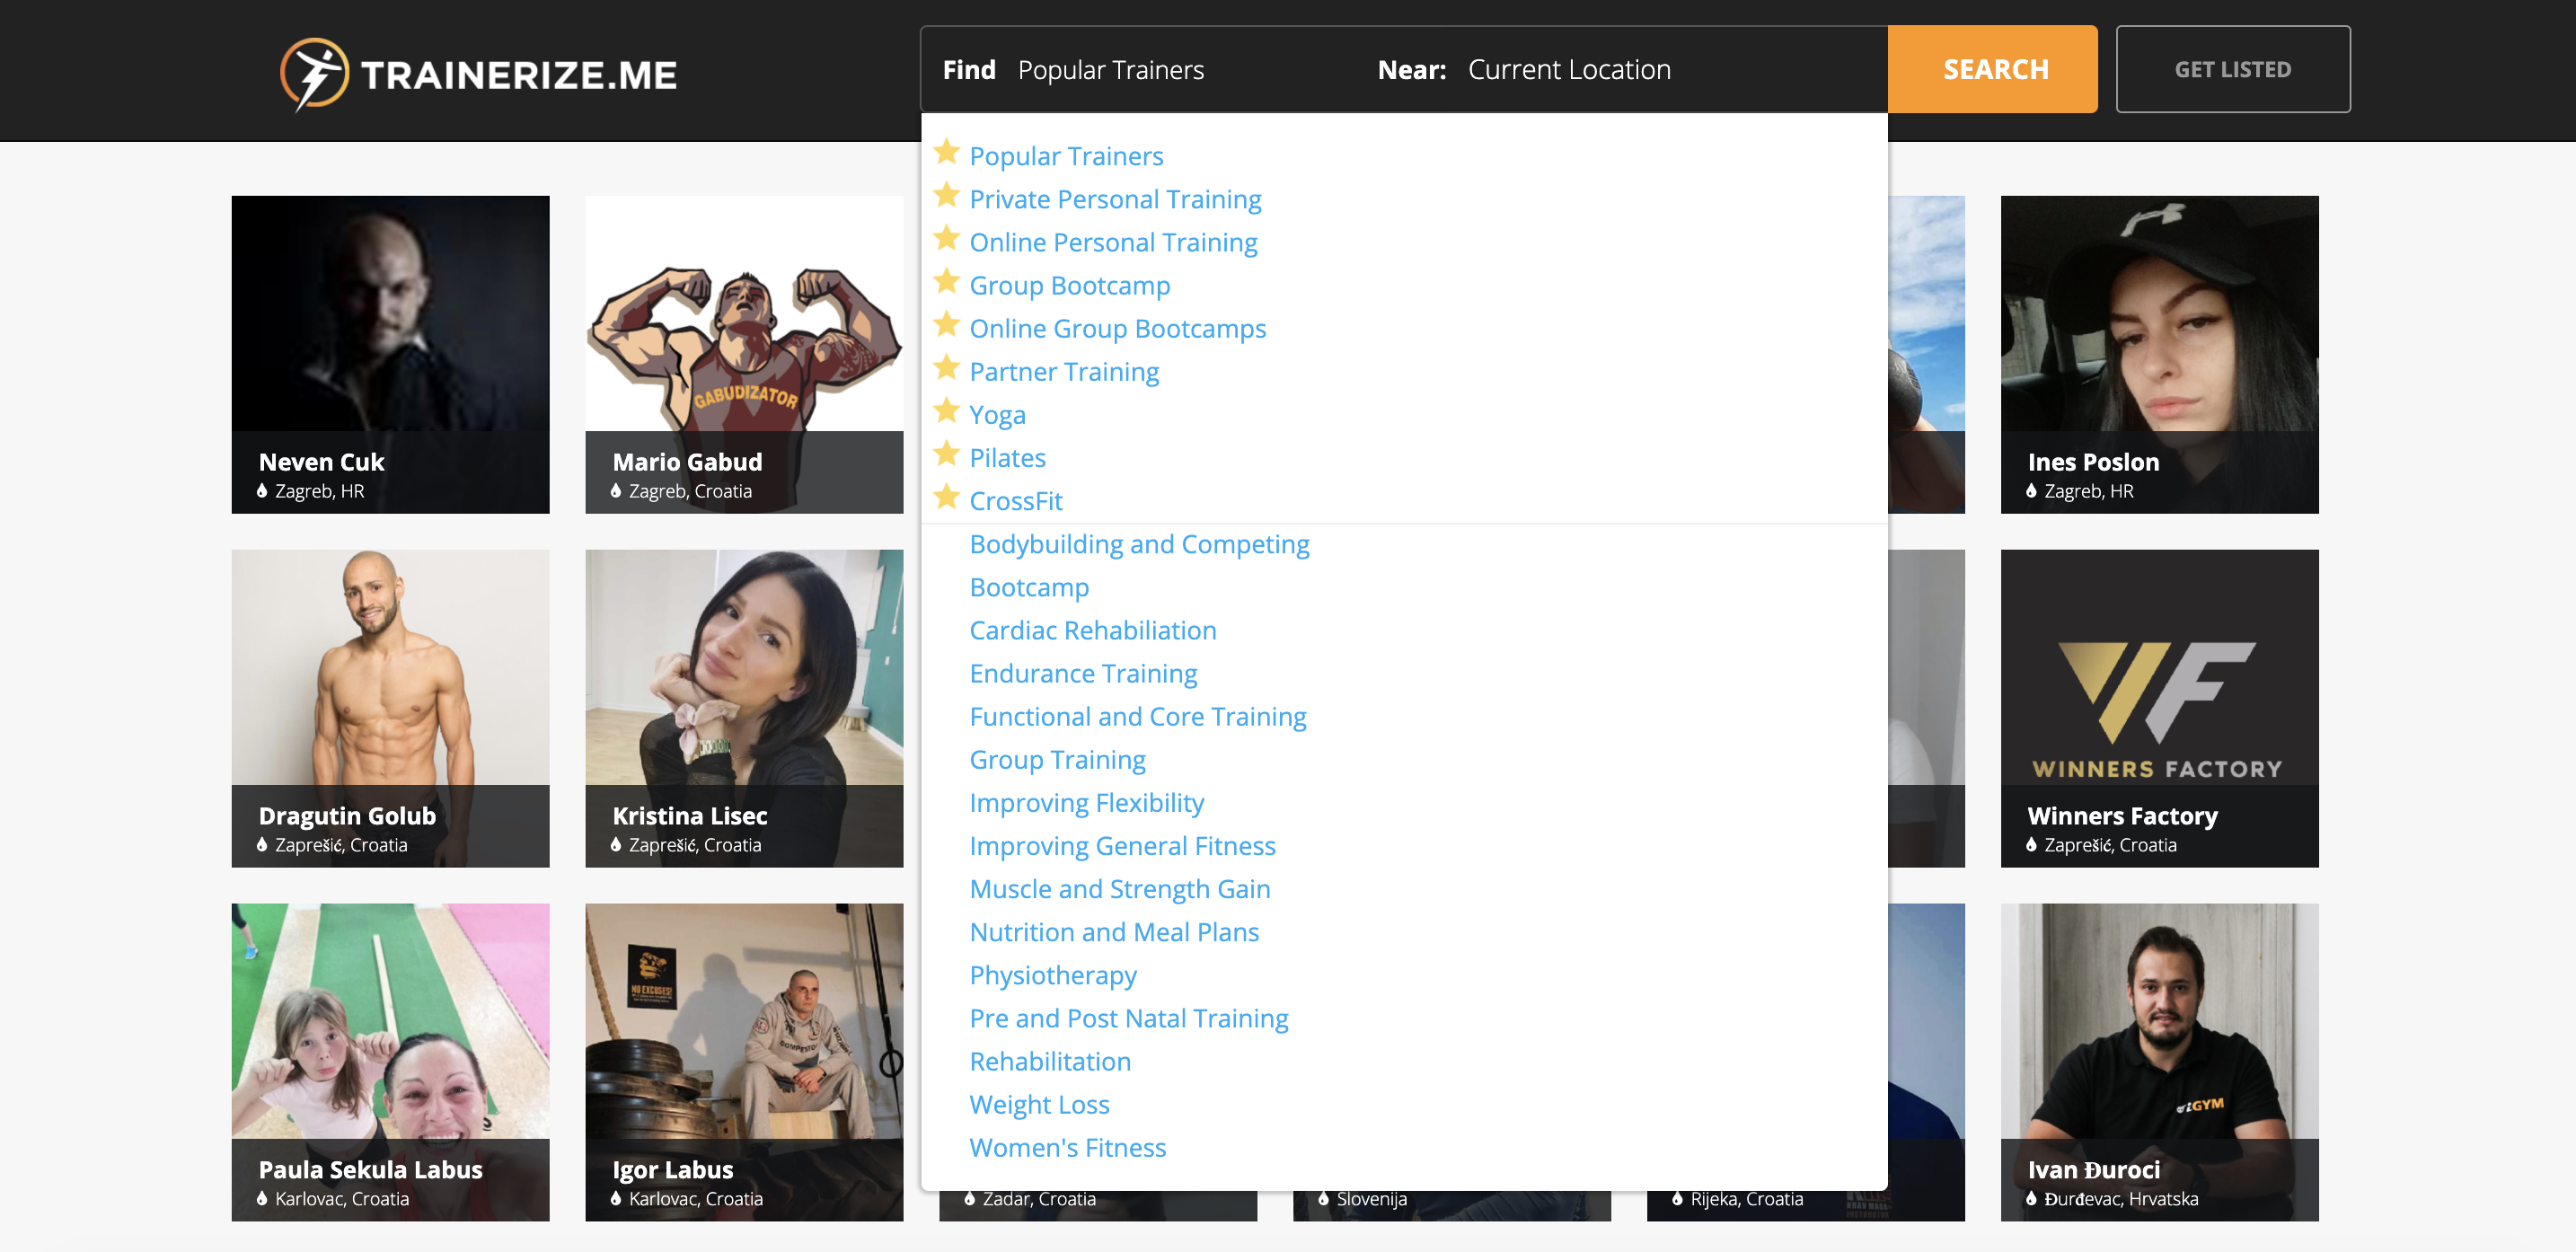
\includegraphics[scale=0.20]{slike/trainerizeme2.PNG} %veličina slike u odnosu na originalnu datoteku i pozicija slike
			\centering
			\caption{Pretraživanje trenera https://www.trainerize.me/}
			\label{fig:promjene}
		\end{figure}
	
		Stranica \href{https://ultimateperformance.com/}{Ultimate Performance (https://ultimateperformance.com/)} nudi gotove planove vježbanja za određene
		svrhe, kao što su gubljenje kilograma, dobivanje mišićne mase i slično, također 
		su programi podijeljeni po spolovima. Također je moguće dogovoriti konzultacije 
		s osobnim trenerima te naručivati personalizirane planove vježbanja.
		
		\begin{figure}[H]
			
\includegraphics[scale=0.20]{slike/ultimateperformance.PNG} %veličina slike u odnosu na originalnu datoteku i pozicija slike
			\centering
			\caption{Početna stranica https://ultimateperformance.com/}
			\label{fig:promjene}
		\end{figure}
		
		\vspace{5mm}
		
		Cilj ovog projekta je razviti programsku podršku za stvaranje web aplikacije
		\textit{"WebGym"} koja će svojim korisnicima uvelike olakšati administrativne 
		poslove vezane uz njihove odlaske u teretanu. Cilj platforme \textit{"WebGym"} 
		je poboljšavanje ukupnog doživljaja teretane, a namijenjena je neregistriranim 
		korisnicima, registriranim korisnicima, trenerima u teretani i voditeljima svake od 
		teretana (jedan voditelj može biti zadužen za više
		teretana i za svaku teretanu može biti zaduženo više voditelja). Za registraciju bilo kojeg od korisnika potrebno je unijeti
		ime, prezime, email adresu i osobne podatke bitne za trenere (visina, težina…) te je PayPal račun opcionalan. 
		
		Prilikom pokretanja sustava (odlaska na početnu stranicu) ukoliko korisnik nije trenutno prijavljen pokazuje se općenita početna stranica. Na toj početnoj stranici u gornjem desnom kutu nalaze se polja za unos korisničkog imena i lozinke te gumb za registraciju korisnika koji se do sada nisu registrirali. Na početnoj stranici se za neregistrirane korisnike nalazi popis najpopularnijih teretana, a svaka teretana u tom popisu ima prikazanu svoju profilnu sliku, ime i adresu teretane.
		
		Za kreiranje novog računa potrebni su sljedeći podaci:

		\begin{packed_item}
			\item Korisničko ime
			\item Ime
			\item Prezime
			\item Broj mobitela
			\item e-mail
		\end{packed_item}
	
		Također opcionalno se mogu unijeti i sljedeći podatci:
		
		\begin{packed_item}
			\item PayPal račun
			\item Visina
			\item Težina
		\end{packed_item}
	
		Pri izradi korisničkog računa moguće je odabrati jednu od tri opcije:
		
		\begin{packed_item}
			\item Korisnik teretana
			\item Admin teretana
			\item Trener
		\end{packed_item}
	
	
	
	
	
		\vspace{5mm}
		
		Mogućnosti nadogradnje ovog projektnog zadatka su mnogobrojne. Moguće je uvesti chat u kojem bi se trenerima i njihovim polaznicima treninga pružila mogućnost izravnog dopisivanja o planu vježbanja, potencijalnim novim ponudama i 
		još mnogo toga. Chat bi se također mogao koristiti između više voditelja iste teretane kako bi mogli koordinirati svoje akcije na platformi ili općenito veze uz poslovanje teretane. Također bi i komunikacija trenera i teretana uvođenjem ove 
		opcije bila uvelike olakšana te bi bila mnogo kvalitetnija. 
		
		Druga potencijalna mogućnost nadogradnje bi bila uvođene online dućana u kojemu 
		bi svaka teretana mogla svojim klijentima nuditi proizvode kao što su suplementi za 
		teretanu, opremu za treniranje i slično. Također bi se mogao uvesti jedinstveni 
		dućan na razini platforme u kojemu bi vlasnici platforme mogli nuditi proizvode ili bi 
		taj dućan mogao biti izveden kao mjesto na kojem dućani koji prodaju suplemente ili 
		opremu za treniranje mogu nuditi svoje proizvode. Ukoliko se dućan odluči izvesti na 
		drugi način u sustavu bi se trebala dodati mogućnost stvaranja dućana te njihovih 
		zaposlenika (to bi bilo izvedeno vrlo slično kao i za teretanu te za voditelje teretana).
		
		
	
		\vspace{5mm}
	
			
		\textit{Za pomoć pogledati reference navedene u poglavlju „Popis literature“, a po potrebi konzultirati sadržaj na internetu koji nudi dobre smjernice u tom pogledu.}
		\eject
		
		\section{Primjeri u \LaTeX u}
		
		\textit{Ovo potpoglavlje izbrisati.}\\

		U nastavku se nalaze različiti primjeri kako koristiti osnovne funkcionalnosti \LaTeX a koje su potrebne za izradu dokumentacije. Za dodatnu pomoć obratiti se asistentu na projektu ili potražiti upute na sljedećim web sjedištima:
		\begin{itemize}
			\item Upute za izradu diplomskog rada u \LaTeX u - \url{https://www.fer.unizg.hr/_download/repository/LaTeX-upute.pdf}
			\item \LaTeX\ projekt - \url{https://www.latex-project.org/help/}
			\item StackExchange za Tex - \url{https://tex.stackexchange.com/}\\
		
		\end{itemize} 	


		
		\noindent \underbar{podcrtani tekst}, \textbf{podebljani tekst}, 	\textit{nagnuti tekst}\\
		\noindent \normalsize primjer \large primjer \Large primjer \LARGE {primjer} \huge {primjer} \Huge primjer \normalsize
				
		\begin{packed_item}
			
			\item  primjer
			\item  primjer
			\item  primjer
			\item[] \begin{packed_enum}
				\item primjer
				\item[] \begin{packed_enum}
					\item[1.a] primjer
					\item[b] primjer
				\end{packed_enum}
				\item primjer
			\end{packed_enum}
			
		\end{packed_item}
		
		\noindent primjer url-a: \url{https://www.fer.unizg.hr/predmet/proinz/projekt}
		
		\noindent posebni znakovi: \# \$ \% \& \{ \} \_ 
		$|$ $<$ $>$ 
		\^{} 
		\~{} 
		$\backslash$ 
		
		\begin{longtabu} to \textwidth {|X[8, l]|X[8, l]|X[16, l]|} %definicija širine tablice, širine stupaca i poravnanje
			
			%definicija naslova tablice
			\hline \multicolumn{3}{|c|}{\textbf{naslov unutar tablice}}	 \\[3pt] \hline
			\endfirsthead
			
			%definicija naslova tablice prilikom prijeloma
			\hline \multicolumn{3}{|c|}{\textbf{naslov unutar tablice}}	 \\[3pt] \hline
			\endhead
			
			\hline 
			\endlastfoot
			
			\rowcolor{LightGreen}IDKorisnik & INT	&  	Lorem ipsum dolor sit amet, consectetur adipiscing elit, sed do eiusmod  	\\ \hline
			korisnickoIme	& VARCHAR &   	\\ \hline 
			email & VARCHAR &   \\ \hline 
			ime & VARCHAR	&  		\\ \hline 
			\cellcolor{LightBlue} primjer	& VARCHAR &   	\\ \hline 
			
		\end{longtabu}
		

		\begin{table}[H]
			
			\begin{longtabu} to \textwidth {|X[8, l]|X[8, l]|X[16, l]|} 
				
				\hline 
				\endfirsthead
				
				\hline 
				\endhead
				
				\hline 
				\endlastfoot
				
				\rowcolor{LightGreen}IDKorisnik & INT	&  	Lorem ipsum dolor sit amet, consectetur adipiscing elit, sed do eiusmod  	\\ \hline
				korisnickoIme	& VARCHAR &   	\\ \hline 
				email & VARCHAR &   \\ \hline 
				ime & VARCHAR	&  		\\ \hline 
				\cellcolor{LightBlue} primjer	& VARCHAR &   	\\ \hline 
				
				
			\end{longtabu}
	
			\caption{\label{tab:referencatablica} Naslov ispod tablice.}
		\end{table}
		
		
		%unos slike
		\begin{figure}[H]
			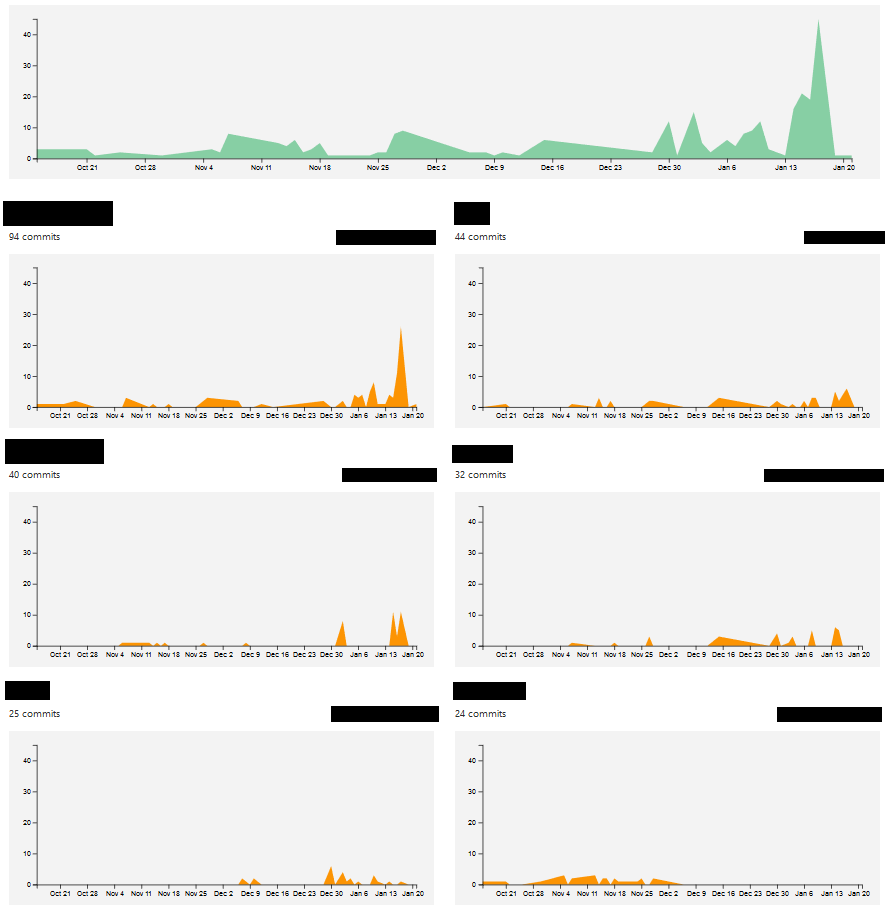
\includegraphics[scale=0.4]{slike/aktivnost.PNG} %veličina slike u odnosu na originalnu datoteku i pozicija slike
			\centering
			\caption{Primjer slike s potpisom}
			\label{fig:promjene}
		\end{figure}
		
		\begin{figure}[H]
			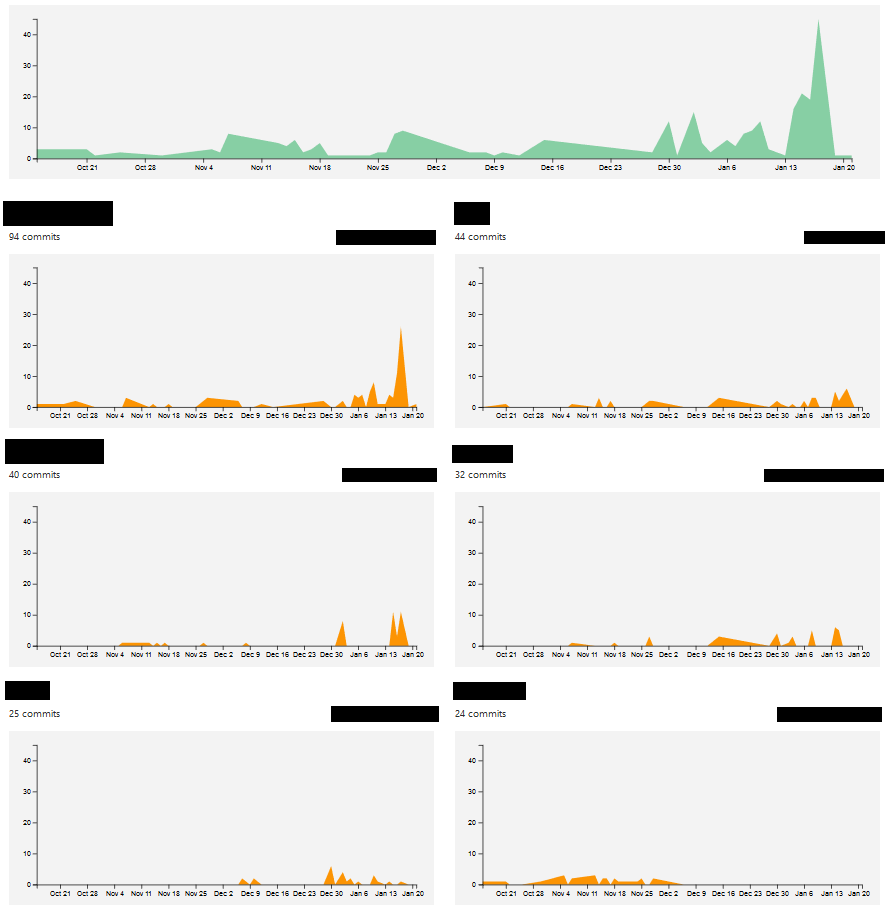
\includegraphics[width=.9\linewidth]{slike/aktivnost.PNG} %veličina u odnosu na širinu linije
			\caption{Primjer slike s potpisom 2}
			\label{fig:promjene2} %label mora biti drugaciji za svaku sliku
		\end{figure}
		
		Referenciranje slike \ref{fig:promjene2} u tekstu.
		
		\eject
		
	
	\chapter{Specifikacija programske potpore}
		
		\section{Funkcionalni zahtjevi}
		
		
		\noindent \textbf{Dionici:}
		
		\begin{packed_enum}
			
			\item Klijent teretane
			\begin{packed_enum}
				
				\item registrirani
				\item neregistrirani
				
			\end{packed_enum}
			\item Trener
			\item Voditelj teretane			
			\item Administrator
			\item Razvojni tim
			
		\end{packed_enum}
		
		\noindent \textbf{Aktori i njihovi funkcionalni zahtjevi:}
		
		
		\begin{packed_enum}
			\item  \underbar{Neregistrirani/neprijavljeni korisnik (inicijator) može:}
			
			\begin{packed_enum}
				
				\item pregledati popis svih teretana na platformi
				\item sortirati spomenuti popis prema sljedećim kriterijima: ime teretane, lokacija, trener
				\item otvoriti početnu stranicu svake teretane na kojoj se nalaze osnovne informacije (radno vrijeme, lokacija, cijena
				članarine…)
				\item izraditi administratorski, voditeljski, trenerski ili korisnički račun s namjerom treniranja u teretani za koje je potrebno navesti ime, prezime i email adresu, dok se može, ali ne mora dodati PayPal račun te je za izradu trenerskog korisničkog računa posebno potrebno navesti posebne podatke poput visine i težine
				
				
			\end{packed_enum}
			
			\item  \underbar{Klijent (inicijator) može:}
			
			\begin{packed_enum}
				
				\item pregledavati i sortirati popis registriranih teretana
				\item pregledavati i mijenjati osobne podatke
				\item izbrisati svoj korisnički račun
				\item plaćati članarine u teretanama putem interneta
				\item pregledavati sve izvršene transakcije u kojima su sudjelovali
				\item pregledavati popis teretana u kojima smiju vježbati, odnosno u kojima su platili članarinu
				\item kupovati planove prehrane i vježbanja od trenera
				\item ugovarati privatne ili grupne treninge
				\item voditi i pratiti napredak u vlastitom planu vježbanja
				
			\end{packed_enum}
			
			\item  \underbar{Trener (inicijator) može:}
			
			\begin{packed_enum}
				
				\item pregledavati i sortirati popis registriranih teretana
				\item pregledavati i mijenjati osobne podatke
				\item izbrisati svoj korisnički račun
				\item objavljivati ponude planova treninga i/ili vježbanja
				\item objavljivati i ugovarati termine privatnih i grupnih treninga u teretanama gdje imaju te ovlasti
				\item pregledavati sve izvršene transakcije u kojima su sudjelovali
				\item pregledavati popis teretana u kojima smiju djelovati, odnosno raditi (voditi treninge, planovi prehrane i sl.)
				\item nuditi usluge treniranja teretanama
				
			\end{packed_enum}
			
			\item  \underbar{Voditelj teretane (inicijator) može:}
			
			\begin{packed_enum}
				
				\item pregledavati i sortirati popis registriranih teretana
				\item pregledavati i mijenjati osobne podatke
				\item izbrisati svoj korisnički račun
				\item stvarati nove teretane u sustavu
				\item davati dozvolu drugim voditeljima da vode neke njegove teretane
				\item mijenjati važne informacije o teretanama (radno vrijeme, lokacija i sl.)
				\item dopuštati registriranim trenerima rad u teretanama koje vodi
				\item vidjeti sve izvršene transakcije na aplikaciji unutar vlastite teretane
				
			\end{packed_enum}
			
			\item  \underbar{Administrator (inicijator) može:}
			
			\begin{packed_enum}
				
				\item pregledavati i sortirati popis registriranih teretana
				\item pregledavati i mijenjati osobne podatke
				\item vidjeti sve korisničke račune
				\item izbrisati svoj korisnički račun
				\item stvarati nove i brisati postojeće teretane u sustavu
				\item pregledati sve izvršene transakcije u aplikaciji
				\item davati dozvolu  voditeljima da vode pojedine teretane
				\item mijenjati važne informacije o teretanama (radno vrijeme, lokacija i sl.)
				\item dopuštati registriranim trenerima rad u teretanama
				
			\end{packed_enum}
			
			
			\item  \underbar{Baza podataka (sudionik):}
			
			\begin{packed_enum}
				
				\item pohranjuje sve podatke o korisnicima
				\item čuva informacije o ulogama pojedinih korisnika
				\item pohranjuje podatke o svim teretanama, njihovim voditeljima, trenerima i članovima
				\item pohranjuje izvršene transakcije
				
			\end{packed_enum}
			
		\end{packed_enum}
		
		\eject
				
			\subsection{Obrasci uporabe}
				
				\textbf{\textit{dio 1. revizije}}
				
				\subsubsection{Opis obrazaca uporabe}

					\noindent \underbar{\textbf{UC1 - Pregled teretana}}
					\begin{packed_item}
	
						\item \textbf{Glavni sudionik: }neregistrirani korisnik, klijent, trener, voditelj teretane i administrator
						\item  \textbf{Cilj:} Pregled teretana
						\item  \textbf{Preduvjet:} -
						\item  \textbf{Opis osnovnog tijeka:}
						
						\item[] \begin{packed_enum}
	
							\item Prikazan popis teretana
							\item Korisnik može tražit teretane (prema nekim kriterijima - search)
							\item Korisnik može birati teretanu o kojoj će dobiti informacije
						\end{packed_enum}
						\end{packed_item}
						
						
						\noindent \underbar{\textbf{UC2 - Registracija korisnika}}
					\begin{packed_item}
	
						\item \textbf{Glavni sudionik: }Neregistrirani korisnik
						\item  \textbf{Cilj:} Izrada korisničkog računa kojim korisnik dobiva dodatne funkcionalnosti sustava
						\item  \textbf{Sudionici:} Baza podataka
						\item  \textbf{Preduvjet:} -
						\item  \textbf{Opis osnovnog tijeka:}
						
						\item[] \begin{packed_enum}
	
							\item Neprijavljeni korisnik odabire opciju registracije
							\item Neprijavljeni korisnik unosi potrebne podatke
							\item Korisnik prima obavijest o uspješnoj registraciji
						\end{packed_enum}
					
						\item  \textbf{Opis mogućih odstupanja:}
						
						\item[] \begin{packed_item}
	
							\item[-]
							Odabir zauzetog korisničkog imena ili e-maila, odabir nepostojećeg e-maila ili nedozvoljen format unosa nekog od podataka
							\item[] \begin{packed_enum}
								
								\item Sustav neprijavljenom korisniku šalje objavu o neuspješnoj registraciji te ga vraća na početnu stranicu za registraciju
								\item Korisnik mijenja neispravne podatke i završava unos ili odustaje od registriranja
								
							\end{packed_enum}
						\end{packed_item}
					\end{packed_item}
					
					\noindent \underbar{\textbf{UC3 - Prijava u sustav}}
					\begin{packed_item}
	
						\item \textbf{Glavni sudionik: }Klijent
						\item  \textbf{Cilj:} Dobiti pristup korisničkom sučelju
						\item  \textbf{Sudionici:} Baza podataka
						\item  \textbf{Preduvjet:} Registracija
						\item  \textbf{Opis osnovnog tijeka:}
						
						\item[] \begin{packed_enum}
	
							\item Unos korisničkog imena i lozinke
							\item Potvrda o ispravnosti unesenih podataka
							\item Pristup korisničkim funkcionalnostima
						\end{packed_enum}
					
						\item  \textbf{Opis mogućih odstupanja:}
						
						\item[] \begin{packed_item}
	
							\item[-]
							Neispravno korisničko ime i/ili lozinka
							\item[] \begin{packed_enum}
								
								\item Sustav obavještava korisnika o neuspješnom upisu i vraća ga na stranicu za prijavu
							\end{packed_enum}
						git it \end{packed_item}
					\end{packed_item}
					
					\noindent \underbar{\textbf{UC4 - Pregled osobnih podataka}}
					\begin{packed_item}
	
						\item \textbf{Glavni sudionik: }Klijent
						\item  \textbf{Cilj:} Pregledati osobne podatke korisnika
						\item  \textbf{Sudionici:} Baza podataka
						\item  \textbf{Preduvjet:} Klijent je prijavljen
						\item  \textbf{Opis osnovnog tijeka:}
						
						\item[] \begin{packed_enum}
	
							\item Klijent odabire opciju "Osobni podaci"
							\item Aplikacija prikazuje osobne podatke korisnika
						\end{packed_enum}
					\end{packed_item}
					
					
					\noindent \underbar{\textbf{UC5 - Promjena osobnih podataka}}
					\begin{packed_item}
	
						\item \textbf{Glavni sudionik: }Klijent, trener, voditelj, administrator
						\item  \textbf{Cilj:} Promijeniti osobne podatke
						\item  \textbf{Sudionici:} Baza podataka
						\item  \textbf{Preduvjet:} Korisnik je prijavljen
						\item  \textbf{Opis osnovnog tijeka:}
						
						\item[] \begin{packed_enum}
	
							\item Korisnik odabire opciju promjene osobnih podataka
							\item Korisnik mijenja svoje osobne podatke
							\begin{packed_item}
	
							\item Ako je korsnik prijavljen kao običan korisnik, on može postaviti svoje ciljeve i rezultate
							\item Ako je korisnik prijavljen kao trener, on može uređivati svoju stranicu
						\end{packed_item}
							\item Korisnik bira opciju "Spremi promjenu"
							\item Ažuracija baze podataka
						\end{packed_enum}
					
						\item  \textbf{Opis mogućih odstupanja:}
						
						\item[] \begin{packed_item}
	
							\item[-]
						Korisnik promijeni podatke, ali ne odabere opciju "Spremi promjenu"
							\item[] \begin{packed_enum}
								
								\item Sustav obavještava korisnika da nije spremio podatke prije izlaska iz prozora
							\end{packed_enum}
						\end{packed_item}
					\end{packed_item}
					
					\noindent \underbar{\textbf{UC6 - Brisanje korisničkog računa}}
					\begin{packed_item}
	
						\item \textbf{Glavni sudionik: }Klijent, trener, voditelj, administrator
						\item  \textbf{Cilj:} Izbrisati svoj korisnički račun
						\item  \textbf{Sudionici:} Baza podataka
						\item  \textbf{Preduvjet:} Korisnik je prijavljen
						\item  \textbf{Opis osnovnog tijeka:}
						
						\item[] \begin{packed_enum}
	
							\item Korisnik pregledava osobne podatke
							\item Korisnik bira opciju "Obriši račun"
							\item Korisnik briše račun
							\item Korisnikov račun se briše iz baze podataka
							\item Otvara se početna stranica
						\end{packed_enum}
					\end{packed_item}
					
					\noindent \underbar{\textbf{UC7 - Pregled specifične teretane}}
					\begin{packed_item}
	
						\item \textbf{Glavni sudionik: }Neregistrirani korisnik, klijent, trener, voditelj, administrator
						\item  \textbf{Cilj:} Vidjeti osnovne podatke o teretani i trenere u toj teretani
						\item  \textbf{Sudionici:} Baza podataka
						\item  \textbf{Preduvjet:} -
						\item  \textbf{Opis osnovnog tijeka:}
						
						\item[] \begin{packed_enum}
	
							\item Korisnik odabire željenu teretanu
							\item Prikazuju se voditelji teretane, treneri koji su dio te teretane, lokacija i radno vrijeme te ponuda članarine
						\end{packed_enum}
					\end{packed_item}
					
					\noindent \underbar{\textbf{UC8 - Pregled transakcija}}
					\begin{packed_item}
	
						\item \textbf{Glavni sudionik: }Klijent, trener, voditelj
						\item  \textbf{Cilj:} Pregled transakcija u kojima je korisnik do sada sudjelovao
						\item  \textbf{Sudionici:} Baza podataka
						\item  \textbf{Preduvjet:} Korisnik je prijavljen
						\item  \textbf{Opis osnovnog tijeka:}
						
						\item[] \begin{packed_enum}
	                        \item Korisnik odabire opciju pregleda osobnih podataka
							\item Korisnik odabire opciju pregleda transakcija
							\item Korisnik dobiva prikaz svih transakcija u kojima je sudjelovao
						\end{packed_enum}
					\end{packed_item}
					
					\noindent \underbar{\textbf{UC9 - Pregled određene transakcije}}
					\begin{packed_item}
	
						\item \textbf{Glavni sudionik: }Klijent, trener, voditelj
						\item  \textbf{Cilj:} Pregled sudionika u transakciji, opis usluge, iznos plaćanja u kunama i datum izvršenja transakcije
						\item  \textbf{Sudionici:} Baza podataka
						\item  \textbf{Preduvjet:} Korisnik je prijavljen
						\item  \textbf{Opis osnovnog tijeka:}
						
						\item[] \begin{packed_enum}
							\item Korisnik odabire opciju pregleda transakcija
							\item Korisnik odabire opciju pregleda određene transakcije
							\item Pregled detalja odabrane transakcije
						\end{packed_enum}
					\end{packed_item}
					
					\noindent \underbar{\textbf{UC10 - Učlanjivanje korisnika u određenu teretanu}}
					\begin{packed_item}
	
						\item \textbf{Glavni sudionik: }Klijent
						\item  \textbf{Cilj:} Učlanjivanje korisnika u određenu teretanu (ili lanac teretana)
						\item  \textbf{Sudionici:} Baza podataka
						\item  \textbf{Preduvjet:} Korisnik je prijavljen
						\item  \textbf{Opis osnovnog tijeka:}
						
						\item[] \begin{packed_enum}
	
							\item Korisnik odabire određenu teretanu
							\item Korisniku se prikazuje ponuda vrsta članarina
							\item Korisnik odabire opciju članarine koju želi platiti
						\end{packed_enum}
					
						\item  \textbf{Opis mogućih odstupanja:}
						
						\item[] \begin{packed_item}
	
						\item[-]
						Korisnik pokušava kupiti članarinu u teretani u kojo već ima aktivnu članarinu istog tipa
							\item[] \begin{packed_enum}
								
								\item Sustav obavještava korisnika da već postoji aktivna članarina tog tipa
								\item Vraća ga na stranicu s popisom članarina te teretane
							\end{packed_enum}
						\end{packed_item}
					\end{packed_item}
				
					
				\subsubsection{Dijagrami obrazaca uporabe}
					
					\textit{Prikazati odnos aktora i obrazaca uporabe odgovarajućim UML dijagramom. Nije nužno nacrtati sve na jednom dijagramu. Modelirati po razinama apstrakcije i skupovima srodnih funkcionalnosti.}
				\eject		
				
			\subsection{Sekvencijski dijagrami}
				
				\textbf{\textit{dio 1. revizije}}\\
				
				\textit{Nacrtati sekvencijske dijagrame koji modeliraju najvažnije dijelove sustava (max. 4 dijagrama). Ukoliko postoji nedoumica oko odabira, razjasniti s asistentom. Uz svaki dijagram napisati detaljni opis dijagrama.}
				\eject
	
		\section{Ostali zahtjevi}
		
			\textbf{\textit{dio 1. revizije}}\\
		 
			 \textit{Nefunkcionalni zahtjevi i zahtjevi domene primjene dopunjuju funkcionalne zahtjeve. Oni opisuju \textbf{kako se sustav treba ponašati} i koja \textbf{ograničenja} treba poštivati (performanse, korisničko iskustvo, pouzdanost, standardi kvalitete, sigurnost...). Primjeri takvih zahtjeva u Vašem projektu mogu biti: podržani jezici korisničkog sučelja, vrijeme odziva, najveći mogući podržani broj korisnika, podržane web/mobilne platforme, razina zaštite (protokoli komunikacije, kriptiranje...)... Svaki takav zahtjev potrebno je navesti u jednoj ili dvije rečenice.}
			 
			 
			 
	
	\chapter{Arhitektura i dizajn sustava}
		
		\textbf{\textit{dio 1. revizije}}\\

		\textit{ Potrebno je opisati stil arhitekture te identificirati: podsustave, preslikavanje na radnu platformu, spremišta podataka, mrežne protokole, globalni upravljački tok i sklopovsko-programske zahtjeve. Po točkama razraditi i popratiti odgovarajućim skicama:}
	\begin{itemize}
		\item 	\textit{izbor arhitekture temeljem principa oblikovanja pokazanih na predavanjima (objasniti zašto ste baš odabrali takvu arhitekturu)}
		\item 	\textit{organizaciju sustava s najviše razine apstrakcije (npr. klijent-poslužitelj, baza podataka, datotečni sustav, grafičko sučelje)}
		\item 	\textit{organizaciju aplikacije (npr. slojevi frontend i backend, MVC arhitektura) }		
	\end{itemize}
	
	Arhitektura korištena pri izradi WebGym web aplikacije sastoji se od:
	\begin{itemize}
		\item   Web poslužitelj
		\item 	Web aplikacija
		\item 	Baza podataka		
	\end{itemize}
	
	\begin{figure}[H]
			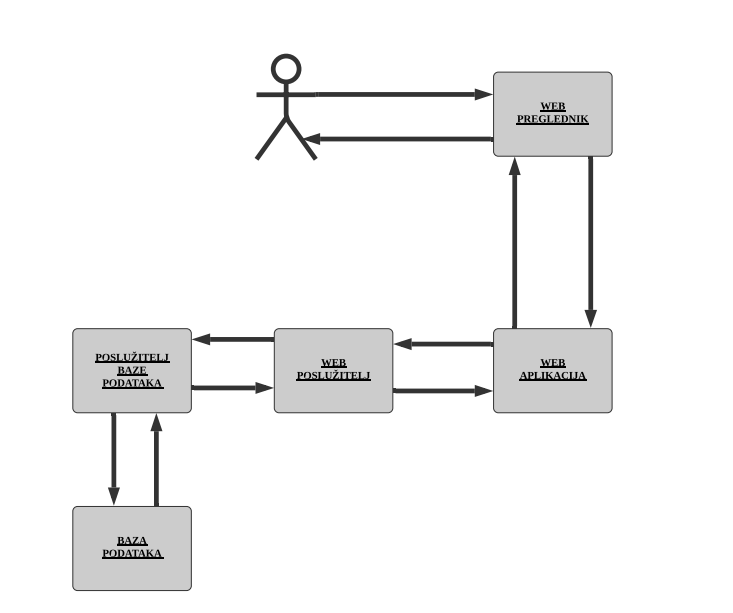
\includegraphics[scale=1.0]{slike/arh.PNG} %veličina slike u odnosu na originalnu datoteku i pozicija slike
			\centering
			\caption{Arhitektura sustava}
			\label{fig:promjene}
		\end{figure}
	Prilikom programiranja sustava prvo se bilo bitno dogovoriti oko korištene arhitekture i tehnologije koja će se za izradu web aplikacije koristiti. Odluke kao što su programski jezik i razvojno okruženje za korištenje same internet aplikacije. Arhitekturu smo odabrali kako bi zadovoljavala mnoge značajke kao što su fleksibilnost, mogućnost nadogradnje, što jeftinije održavanje. Web aplikacije nam se činila kao najlogičniji odabir iz razloga što ne ovisi o uređaju na kojem se prikazuje te se nismo morali opredijeljivati za operacijski sustav u kojem će raditi najefikasnije. Također odabrana arhitektura od korisnika naše web aplikacije zahtjeva samo pristup internet te internetski preglednik što je dostupno većini.  \newline
	\indent Pregled web-stranice te svih podataka i zatraženih medija odvija se uz pomoć \underbar{\textit{web preglednika}}. Web preglednik ima nekoliko uloga, jedna od njih je prikaz stranice na način čitljiv čovjeku. Stoga možemo reći da web preglednik ima funkciju prevoditelja. Također, upravo web preglednik je alat pomoću kojeg korisnik šalje zahtjev web poslužitelju. \newline
	\indent Iduća funkcionalnost je komunkacija s aplikacijom. Tome služi \underbar{\textit{web poslužitelj}} koji je poput motora web aplikacije. Sama komunikacija odvija se pomoću HTTP protokola koji služi za prijenos informacija i komunikaciju na internetu. \newline
	\indent \underbar{\textit{Web aplikacija}} se pokreće pomoću web poslužitelja koji joj prosljeđuje zahjtev, a sama web aplikacija služi za obradu zahtjeva prosljeđenih s web poslužitelja. Web aplikacija ima mogućnost pristupa bazi podataka. Podaci iz baze se kasnije prikazuju korisniku. Za sami prikaz je zaslužen već prije spomenuti web poslužitelj koji vraća korisniku HTML dokument kao odgovor, a čitljivi prikaz korisniku je osiguran pomoću web preglednika. \newline
	\indent Web aplikacija nam se sastoji od front-enda i back-enda. Tehnologija koju smo odabrali za izradu back-enda je Java Spring Boot, dok smo za front-end odabrali React.js. Arhitektura sustava za koju smo se odlučili je MVC odnosno (Model-View-Controller) koncept. \newline
	\indent Glavna korist MVC kocepta je ta što dijelovi aplikacije nisu usko povezani te se lakše testiraju, a i greška u jednom od dijelova neće utjecati na rad ostalih. \newline
	MVC koncept sastoji se od:
	\begin{itemize}
		\item   \textbf{Model} - klase koje opisuju same podatke koji se koriste u aplikaciji. Klase također sadrže i logiku vezanu za te podatke. Podaci u modelu ne ovise o korisničkom sučelju. Model prima ulazne podatke od Controllera.
		\item 	\textbf{View} - omogućuje komunikaciju s korisnikom te definira kako će korisničko sučelje biti prikazano korisniku.
		\item 	\textbf{Controller}	- klase koje kontroliraju komunikaciju korisnika sa aplikacijom. To je sloj aplikacije koji obrađuje korisničke zahtjeve. Controller prihvaća sve ulaze i pretvara ih u naredbe za Model i View.   	
	\end{itemize}

	
		\section{Baza podataka}
		Za potrebe WebGym sustava koristit ćemo relacijsku bazu podataka koja nam pojednostavljuje modeliranje odnosa i scenarija koji se u realnosti dešavaju. Svaka je tablica definirana svojim imenom te skupom atributa koji su nam potrebni za punu funkcionalnost pojma ili odnosa opisanim tablicom. Brza i jednostavna pohrana te pristup samim podacima je zadaća ovog sustava pohranjivanja podataka u bazu. Baza podataka sastoji se od sljedećih entiteta:
		\begin{itemize}
	        	\item 	Korisnik
	        	\item 	Teretana 
	        	\item 	TeretanaLokacija 
	        	\item   Ciljevi
	        	\item 	PlanTreningaIPrehrane
	        	\item 	Članarina
	        	\item 	ČlanarinaKlijent
	        	\item 	Zamolba
	        	\item   PlanKlijent
	        	\item   TeretanaKorisnik
        	\end{itemize}
		
		
		\subsection{Opis tablica}
		\textbf{Korisnik} Ovaj entitet sadržava sve bitne informacije o korisniku WebGym web aplikacije. Sadrži atribute kao što su: korisničko ime, ime, prezime, email, hashiranu lozinku, broj mobitela, broj PayPala, visinu, težinu te ulogu u sustavu. Primarni ključ ovog entiteta je korisničkoIme te je stoga taj atribut boldan u tablici. U ulozi ovise ovlasti koje korisnik u sustavu i u odnosima ima. Ovaj entitet je u vezi \emph{One-to-Many} s entitetom Ciljevi preko korisničkog imena klijenta koji je i sam korisnik, u vezi s \emph{Many-to-Many} entitetom PlanTreningaIPrehrane preko korisničkog imena trenera koji je i sam korisnik, u vezi \emph{One-to-Many} s entitetom ČlanarinaKlijent preko korisničkog imena klijenta, u vezi \emph{One-to-Many} s entitetom  Zamolba korisničkog imena trenera, u vezi \emph{Many-to-Many} s entitetom PlanKlijent preko korisničkog imena klijenta te u vezi \emph{Many-to-Many} s entitetom TeretanaKorisnik preko korisničkog imena trenera ili voditelja koji su i sami korisnici.
				
				
    			\begin{longtabu} to \textwidth {|X[10, l]|X[6, l]|X[20, l]|}
    					
    				\hline \multicolumn{3}{|c|}{\textbf{Korisnik}}	 \\[3pt] \hline
    				\endfirsthead
    					
    				\hline \multicolumn{3}{|c|}{\textbf{Korisnik}}	 \\[3pt] \hline
    				\endhead
    					
    				\hline 
    				\endlastfoot
    					
    					\textbf{korisničkoIme}  & VARCHAR	&  	jedinstveno ime korisnika 	\\ \hline
    					ime	& VARCHAR & ime korisnika  	\\ \hline 
    					prezime & VARCHAR & prezime korisnika   \\ \hline 
    					email & VARCHAR	&  	email korisnika s kojim je napravio račun	\\ \hline 
    					lozinka	& VARCHAR & hash korisnikove lozinke za prijavu  	\\ \hline
    					brojMobitela	& VARCHAR & korisnikov broj mobitela  	\\ \hline
    					PayPal	& VARCHAR & korisnikov PayPal za plaćanje usluga  	\\ \hline
    					visina	& INT & korisnikova težina  	\\ \hline
    					težina	& INT & korisnikova visina  	\\ \hline
    					uloga	& VARCHAR & korisnikova uloga u sustavu  	\\ \hline
					
					
				\end{longtabu}
				
				\textbf{Teretana} ovaj entitet sadrži sve bitne informacije o lancu teretani. Sadrži atribute: id, ime, opis te email, a ovaj je entitet u vezi \emph{One-to-Many} s entitetom TeretanaLokacija preko jedinstvenog brojčanog identifikatora teretane te u vezi \emph{One-to-Many} s entitetom članarina preko jedinstvenog brojčanog identifikatora teretane. Primarni ključ ovog entiteta je id te je stoga taj atribut boldan u tablici.
				\begin{longtabu} to \textwidth {|X[10, l]|X[6, l]|X[20, l]|}
    					
    				\hline \multicolumn{3}{|c|}{\textbf{Teretana}}	 \\[3pt] \hline
    				\endfirsthead
    					
    				\hline \multicolumn{3}{|c|}{\textbf{Teretana}}	 \\[3pt] \hline
    				\endhead
    					
    				\hline 
    				\endlastfoot
    					
    					\textbf{id}  & INT	&  	jedinstveni brojčani identifikator teretane 	\\ \hline
    					ime	& VARCHAR & ime teretane  	\\ \hline 
    					opis & VARCHAR & opis teretane   \\ \hline 
    					email & VARCHAR	&  	e mail teretane	\\ \hline 
					
					
				\end{longtabu}
				
			\textbf{TeretanaLokacija} ovaj entitet sadrži sve bitne informacije o pojedinoj teretani. Sadrži atribute: id,id lanca teretani, država u kojoj se nalazi, grad u kojem se nalazi, ulica u kojoj se nalazi, početak ranog vremena teretane, kraj radnog vremena teretane te broj telefona teretane, a ovaj je entitet u vezi \emph{Many-to-One} s entitetom Teretana preko jedinstvenog brojčanog identifikatora teretane, u vezi \emph{One-to-Many} s entitetom Zamolba preko jedinstvenog brojčanog identifikatora pojedine teretane te je u vezi \emph{One-to-Many} s entitetom TeretanaKorisnik preko jedinstvenog brojčanog identifikatora pojedine teretane. Primarni ključ ovog entiteta je id te je stoga taj atribut boldan u tablici, dok je idTeretana strani ključ te je stoga taj atribut pisan formatom italic u tablici.
			\begin{longtabu} to \textwidth {|X[10, l]|X[6, l]|X[20, l]|}
    					
    				\hline \multicolumn{3}{|c|}{\textbf{TeretanaLokacija}}	 \\[3pt] \hline
    				\endfirsthead
    					
    				\hline \multicolumn{3}{|c|}{\textbf{TeretanaLokacija}}	 \\[3pt] \hline
    				\endhead
    					
    				\hline 
    				\endlastfoot
    					
    					\textbf{id}  & INT	&  	jedinstveni brojčani identifikator pojedine teretane 	\\ \hline
    					\textit{idTeretana}	& INT & jedinstveni brojčani identifikator lanca teretani (Teretana.id)  	\\ \hline 
    					država & VARCHAR & država u kojoj se teretana nalazi   \\ \hline 
    					grad & VARCHAR	&  	grad u kojem se teretana nalazi	\\ \hline 
    					ulica	& VARCHAR & ulica u kojoj se teretana nalazi  	\\ \hline
    					radnoVrijemePočetak	& TIME & vrijeme početka rada teretane  	\\ \hline
    					radnoVrijemeKraj	& TIME & vrijeme kraja rada teretane  	\\ \hline
    					telefon	& VARCHAR & broj na koji se teretana može nazvati  	\\ \hline
					
					
			\end{longtabu}
			
			\textbf{Ciljevi} ovaj entitet sadrži sve važne informacije o ciljevima samog klijenta. Sadrži atribute: id,korisničko ime klijenta te opis cilja, a ovaj je entitet u vezi \emph{Many-to-One} s entitetom Korisnik preko korisničkog imena.Primarni ključ ovog entiteta je id te je stoga taj atribut boldan u tablici, dok je korisničkoImeKlijent strani ključ te je stoga taj atribut pisan formatom italic u tablici.
			\begin{longtabu} to \textwidth {|X[10, l]|X[6, l]|X[20, l]|}
    					
    				\hline \multicolumn{3}{|c|}{\textbf{Ciljevi}}	 \\[3pt] \hline
    				\endfirsthead
    					
    				\hline \multicolumn{3}{|c|}{\textbf{Ciljevi}}	 \\[3pt] \hline
    				\endhead
    					
    				\hline 
    				\endlastfoot
    					
    					\textbf{id}  & INT	&  	jedinstveni brojčani identifikator cilja 	\\ \hline
    					\textit{korisničkoImeKlijent}	& VARCHAR & jedinstveni brojčani identifikator klijenta koji cilj obavlja (Korisnik.korisničkoIme)  	\\ \hline 
    					opis & VARCHAR & opis cilja   \\ \hline 
    					obavljeno & BOOLEAN	& je li cilj obavljen	\\ \hline 
					
					
			\end{longtabu}
			
			
			\textbf{PlanTreningaIPrehrane} ovaj entitet sadrži sve važne informacije o planu treninga i prehrane. Korisnik može kupiti trening te onda ima individualni pristup trenera, ili može samo kupiti plan te dobiti gotov file sa treninzima i preporučenim načinom prehrane. Sadrži atribute: id,korisničko ime trenera, opis plana, datum početka plana, datum isteka plana te atribut koji nam govori je li trening u pitanju, a ovaj je entitet u vezi \emph{Many-to-Many} s entitetom Korisnik preko korisničkog imena. Primarni ključ ovog entiteta je id te je stoga taj atribut boldan u tablici, dok je korisničkoImeTrener strani ključ te je stoga taj atribut pisan formatom italic u tablici.
			\begin{longtabu} to \textwidth {|X[10, l]|X[6, l]|X[20, l]|}
    					
    				\hline \multicolumn{3}{|c|}{\textbf{PlanTreningaIPrehrane}}	 \\[3pt] \hline
    				\endfirsthead
    					
    				\hline \multicolumn{3}{|c|}{\textbf{PlanTreningaIPrehrane}}	 \\[3pt] \hline
    				\endhead
    					
    				\hline 
    				\endlastfoot
    					
    					\textbf{id}  & INT	&  	jedinstveni brojčani identifikator plana treninga i prehrane 	\\ \hline
    					\textit{korisničkoImeTrener} 	& VARCHAR & jedinstveni brojčani identifikator trenera čiji je plan (Korisnik.korisničkoIme)  	\\ \hline 
    					opis & VARCHAR & opis plana treninga i prehrane   \\ \hline 
    					datumPočetka & TIMESTAMP & vrijeme početka plana   \\ \hline
    					datumIsteka & TIMESTAMP & vrijeme kraja plana   \\ \hline
    					cijena & DECIMAL & cijena plana   \\ \hline
    					jeLiTrening & BOOLEAN	& je li plan individalni plan, inače je samo kupljeni gotovi plan treninga i prehrane	\\ \hline
					
					
			\end{longtabu}
			
			\textbf{Članarina} ovaj entitet sadrži sve važne informacije o članarini u teretani.  Sadrži atribute: id,id pojedine teretane, cijena članarine, opis te trajanje, a ovaj je entitet u vezi \emph{Many-to-One} s entitetom Teretana preko jedinstvenog brojčanog identifikatora teretane te je u vezi \emph{One-to-Many} s entitetom ČlanarinaKlijent preko jedinstvenog brojčanog identifikatora članarine. Primarni ključ ovog entiteta je id te je stoga taj atribut boldan u tablici, dok je idTeretana strani ključ te je stoga taj atribut pisan formatom italic u tablici.
			\begin{longtabu} to \textwidth {|X[10, l]|X[6, l]|X[20, l]|}
    					
    				\hline \multicolumn{3}{|c|}{\textbf{Članarina}}	 \\[3pt] \hline
    				\endfirsthead
    					
    				\hline \multicolumn{3}{|c|}{\textbf{Članarina}}	 \\[3pt] \hline
    				\endhead
    					
    				\hline 
    				\endlastfoot
    					
    					\textbf{id}  & INT	&  	jedinstveni brojčani identifikator članarine 	\\ \hline
    					\textit{idTeretana}  	& INT & jedinstveni brojčani identifikator trenere koja nudi članarinu (Teretana.id)  	\\ \hline
    					cijena & DECIMAL & cijena članarine   \\ \hline
    					opis & VARCHAR & opis članarine (što se članarina uključuje)   \\ \hline
    					trajanje & INTERVAL & trajanje članarine   \\ \hline
					
					
			\end{longtabu}
			
			\textbf{ČlanarinaKlijent} ovaj entitet sadrži sve važne informacije o članarini koju klijent posjeduje. Sadrži atribute: id,korisničko ime klijenta, id članarine koju teretana nudi, datum početka te dazum isteka trajanja članarine, a ovaj je entitet u vezi \emph{Many-to-One} s entitetom Korisnik preko korisničkog imena klijenta te je u vezi \emph{Many-to-One} s entitetom Članarina preko jedinstvenog brojčanog identifikatora članarine. Primarni ključ ovog entiteta je id te je stoga taj atribut boldan u tablici, dok su korisničkoImeKlijent i idČlanarina strani ključevi te su stoga ti atributi pisani formatom italic u tablici.
			\begin{longtabu} to \textwidth {|X[10, l]|X[6, l]|X[20, l]|}
    					
    				\hline \multicolumn{3}{|c|}{\textbf{ČlanarinaKlijent}}	 \\[3pt] \hline
    				\endfirsthead
    					
    				\hline \multicolumn{3}{|c|}{\textbf{ČlanarinaKlijent}}	 \\[3pt] \hline
    				\endhead
    					
    				\hline 
    				\endlastfoot
    					
    					\textbf{id}  & INT	&  	jedinstveni brojčani identifikator članarine koju klijent posjeduje 	\\ \hline
    					\textit{korisničkoImeKlijent}  	& VARCHAR & korisničko ime klijenta koji posjeduje članarinu (Korisnik.korisničkoIme)  	\\ \hline
    					\textit{idČlanarina}  	& INT & jedinstveni brojčani identifikator članarine (Članarina.id)    \\ \hline
					    datumPočetka & TIMESTAMP & datum početka trajanja članarine   \\ \hline
    					datumIsteka & TIMESTAMP & datum kraja trajanja članarine   \\ \hline
					
			\end{longtabu}
			
			\textbf{Zamolba} ovaj entitet sadrži sve važne informacije o prijavi za posao koju trener šalje pojedinoj teretani. Sadrži atribute: id,korisničko ime trenera, id pojedine teretane u kojoj se trener za posao prijavljuje, te opis prijave, a ovaj je entitet u vezi \emph{Many-to-One} s entitetom Korisnik preko korisničkog imena trenera te je u vezi \emph{Many-to-One} s entitetom Teretana preko jedinstvenog brojčanog identifikatora teretane. Primarni ključ ovog entiteta je id te je stoga taj atribut boldan u tablici, dok su korisničkoImeTrener i idTeretana strani ključevi te su stoga ti atributi pisani formatom italic u tablici.
			\begin{longtabu} to \textwidth {|X[10, l]|X[6, l]|X[20, l]|}
    					
    				\hline \multicolumn{3}{|c|}{\textbf{Zamolba}}	 \\[3pt] \hline
    				\endfirsthead
    					
    				\hline \multicolumn{3}{|c|}{\textbf{Zamolba}}	 \\[3pt] \hline
    				\endhead
    					
    				\hline 
    				\endlastfoot
    					
    					\textbf{id}  & INT	&  	jedinstveni brojčani identifikator prijave 	\\ \hline
    					\textit{korisničkoImeTrener} 	& VARCHAR & korisničko ime trenera koji se prijavljuje za posao u teretani (Korisnik.korisničkoIme)  	\\ \hline
    					\textit{idTeretana}  	& INT & jedinstveni identifikator teretane u koju se prijavljuje (TeretanaLokacija.id)    \\ \hline
					    opis & VARCHAR & opis prijave za posao   \\ \hline
    					dozvola & BOOLEAN & je li treneru odobren rad u teretani   \\ \hline
					
			\end{longtabu}
			
			\textbf{PlanKlijent} ovaj entitet sadrži sve važne informacije o planu prehrane i treninga kojeg klijent posjeduje. Sadrži atribute: id, id plana, korisničko ime klijenta, te datum kupnje, a ovaj je entitet u vezi \emph{Many-to-One} s entitetom Korisnik preko korisničkog imena klijenta te je u vezi  \emph{Many-to-One} s entitetom PlanTreningaIPrehrane preko jedinstvenog brojčanog identifikatora plana. Primarni ključ ovog entiteta je id te je stoga taj atribut boldan u tablici, dok su korisničkoImeKlijent i idPlan strani ključevi te su stoga ti atributi pisani formatom italic u tablici.
			\begin{longtabu} to \textwidth {|X[11, l]|X[6, l]|X[20, l]|}
    					
    				\hline \multicolumn{3}{|c|}{\textbf{PlanKlijent}}	 \\[3pt] \hline
    				\endfirsthead
    					
    				\hline \multicolumn{3}{|c|}{\textbf{PlanKlijent}}	 \\[3pt] \hline
    				\endhead
    					
    				\hline 
    				\endlastfoot
    					
    					\textbf{id}  & INT	&  	jedinstveni brojčani identifikator plana kojeg klijent posjeduje 	\\ \hline
    					\textit{idPlan} 	& INT & jedinstveni brojčani identifikator plana treninga i prehrane (PlanTreningaIPrehrane.id)  	\\ \hline
    					\textit{korisničkoImeKlijent}  & VARCHAR & korisničko ime klijenta koji plan posjeduje (Korisnik.korisničkoIme) \\ \hline
					    datumKupnje & TIMESTAMP & datum kupnje plana   \\ \hline
		    \end{longtabu}
			
			\textbf{TeretanaKorisnik} ovaj entitet sadrži sve važne informacije o korisniku koji radi u teretani kao voditelj ili kao trener. Sadrži atribute: id, id pojedine teretane, korisničko ime korisnika, te datum početka rada, a ovaj je entitet u vezi \emph{Many-to-One} s entitetom Korisnik preko korisničkog imena korisnika te je u vezi \emph{Many-to-One} s entitetom TeretanaLokacija preko jedinstvenog brojčanog identifikatora pojedine teretane. Primarni ključ ovog entiteta je id te je stoga taj atribut boldan u tablici, dok su idTeretana i korisničkoImeKorisnik strani ključevi te su stoga ti atributi pisani formatom italic u tablici.
			\begin{longtabu} to \textwidth {|X[11, l]|X[6, l]|X[20, l]|}
    					
    				\hline \multicolumn{3}{|c|}{\textbf{TeretanaKorisnik}}	 \\[3pt] \hline
    				\endfirsthead
    					
    				\hline \multicolumn{3}{|c|}{\textbf{TeretanaKorisnik}}	 \\[3pt] \hline
    				\endhead
    					
    				\hline 
    				\endlastfoot
    					
    					\textbf{id}  & INT	&  	jedinstveni brojčani identifikator odnosa korisnika i teretane 	\\ \hline
    					\textit{idTeretana} 	& INT & jedinstveni brojčani identifikator plana treninga i prehrane (TeretanaLokacija.id)  	\\ \hline
    					\textit{korisničkoImeKorisnik}  & VARCHAR & korisničko ime trenera ili voditelja u teretani (Korisnik.korisničkoIme)   \\ \hline
					    datumPočetkaRada & TIMESTAMP & datum zaposlenja trenera u teretani   \\ \hline
					
			\end{longtabu}
			
			
			\subsection{Dijagram baze podataka}
				\textit{ U ovom potpoglavlju potrebno je umetnuti dijagram baze podataka. Primarni i strani ključevi moraju biti označeni, a tablice povezane. Bazu podataka je potrebno normalizirati. Podsjetite se kolegija "Baze podataka".}
				
				\begin{figure}[H]
					\hspace*{-1.5cm}
					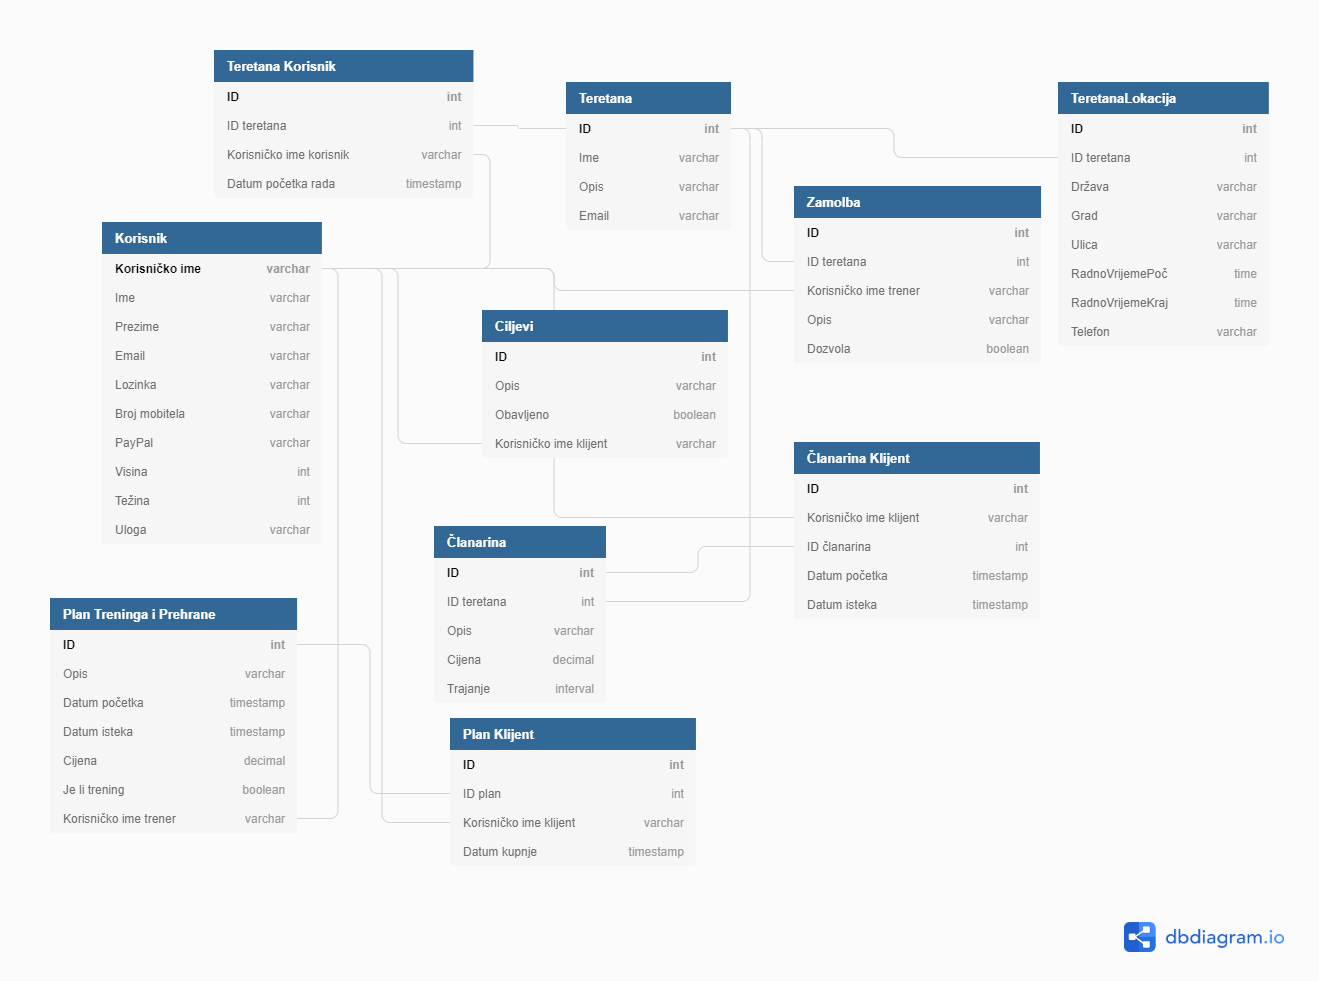
\includegraphics[scale=0.4]{dijagrami/dijagram_baze_podataka.PNG} %veličina slike u odnosu na originalnu datoteku i pozicija slike
					\centering
					\caption{E-R dijagram baze podataka}
					\label{fig:promjene}
				\end{figure}
			
			\eject
			
			
		\section{Dijagram razreda}
		
			\textit{Potrebno je priložiti dijagram razreda s pripadajućim opisom. Zbog preglednosti je moguće dijagram razlomiti na više njih, ali moraju biti grupirani prema sličnim razinama apstrakcije i srodnim funkcionalnostima.}\\
			
			\textbf{\textit{dio 1. revizije}}\\
			
			\textit{Prilikom prve predaje projekta, potrebno je priložiti potpuno razrađen dijagram razreda vezan uz \textbf{generičku funkcionalnost} sustava. Ostale funkcionalnosti trebaju biti idejno razrađene u dijagramu sa sljedećim komponentama: nazivi razreda, nazivi metoda i vrste pristupa metodama (npr. javni, zaštićeni), nazivi atributa razreda, veze i odnosi između razreda.}\\
			
			\textbf{\textit{dio 2. revizije}}\\			
			
			\textit{Prilikom druge predaje projekta dijagram razreda i opisi moraju odgovarati stvarnom stanju implementacije}
			
			
			
			\eject
		
		\section{Dijagram stanja}
			
			
			\textbf{\textit{dio 2. revizije}}\\
			
			\textit{Potrebno je priložiti dijagram stanja i opisati ga. Dovoljan je jedan dijagram stanja koji prikazuje \textbf{značajan dio funkcionalnosti} sustava. Na primjer, stanja korisničkog sučelja i tijek korištenja neke ključne funkcionalnosti jesu značajan dio sustava, a registracija i prijava nisu. }
			
			
			\eject 
		
		\section{Dijagram aktivnosti}
			
			\textbf{\textit{dio 2. revizije}}\\
			
			 \textit{Potrebno je priložiti dijagram aktivnosti s pripadajućim opisom. Dijagram aktivnosti treba prikazivati značajan dio sustava.}
			
			\eject
		\section{Dijagram komponenti}
		
			\textbf{\textit{dio 2. revizije}}\\
		
			 \textit{Potrebno je priložiti dijagram komponenti s pripadajućim opisom. Dijagram komponenti treba prikazivati strukturu cijele aplikacije.}
	\chapter{Implementacija i korisničko sučelje}
		
		
		\section{Korištene tehnologije i alati}
		
			\textbf{\textit{dio 2. revizije}}
			
			 \textit{Detaljno navesti sve tehnologije i alate koji su primijenjeni pri izradi dokumentacije i aplikacije. Ukratko ih opisati, te navesti njihovo značenje i mjesto primjene. Za svaki navedeni alat i tehnologiju je potrebno \textbf{navesti internet poveznicu} gdje se mogu preuzeti ili više saznati o njima}.
			
			
			\eject 
		
	
		\section{Ispitivanje programskog rješenja}
			
			\textbf{}\\
			
			 \textit{U ovom poglavlju je potrebno opisati provedbu ispitivanja implementiranih funkcionalnosti na razini komponenti i na razini cijelog sustava s prikazom odabranih ispitnih slučajeva. Studenti trebaju ispitati temeljnu funkcionalnost i rubne uvjete.}
	
			
			\subsection{Ispitivanje komponenti}
			\textit{Potrebno je provesti ispitivanje jedinica (engl. unit testing) nad razredima koji implementiraju temeljne funkcionalnosti. Razraditi \textbf{minimalno 6 ispitnih slučajeva} u kojima će se ispitati redovni slučajevi, rubni uvjeti te izazivanje pogreške (engl. exception throwing). Poželjno je stvoriti i ispitni slučaj koji koristi funkcionalnosti koje nisu implementirane. Potrebno je priložiti izvorni kôd svih ispitnih slučajeva te prikaz rezultata izvođenja ispita u razvojnom okruženju (prolaz/pad ispita). }
			
			Za ispitivanje razrednih funkcija koje implementiraju temeljne funkcionalnosti koristili smo MockMvc. MockMvc je razred definiran u javi pomoću kojeg možemo kontrolerima poslati lažne HTTP zahtjeve i testirati njihovo  ponašanje bez pokretanja kontrolera unutar poslužitelja.U nastavku će biti prikazani neke od metoda koje smo testirali i odlučili prikazati.
			
			 \noindent \underbar{\textbf{1. Dohvati sve teretane}}
			 
             Ovdje smo testirali pokušaj dohvaćanja teretana odlaskom na /getGyms.

			\begin{figure}[H]
    			\hspace*{-1.5cm}
    			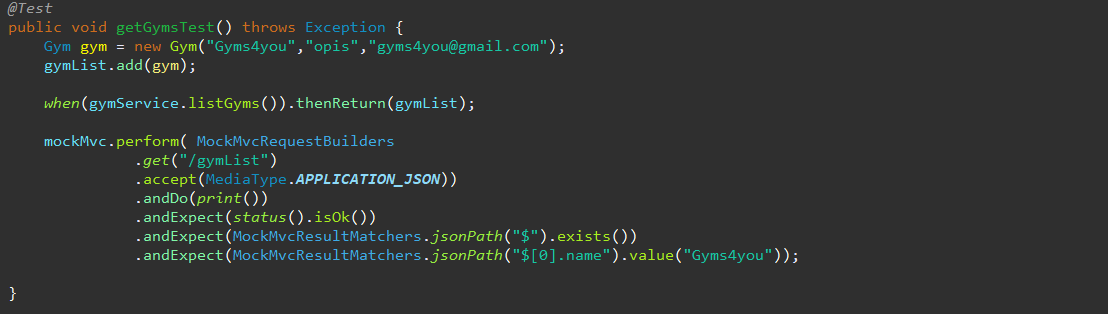
\includegraphics[scale=0.5]{slike/getGyms.PNG} %veličina slike u odnosu na originalnu datoteku i pozicija slike
    			\centering
    			\label{fig:promjene}
    	    \end{figure}
	

			\noindent \underbar{\textbf{2. Dodaj novu teretanu}}
			
            Ovdje smo testirali pokušaj dodavanja nove teretane odlaskom na /addGym  dok smo ulogirani kao role owner.

			\begin{figure}[H]
    			\hspace*{-1.5cm}
    			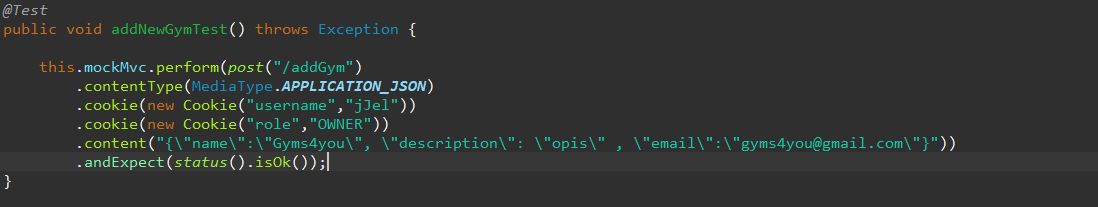
\includegraphics[scale=0.5]{slike/addNewGym.PNG} %veličina slike u odnosu na originalnu datoteku i pozicija slike
    			\centering
    			\label{fig:promjene}
    	    \end{figure}
	

			\noindent \underbar{\textbf{3. Dohvati trenerovu teretanu}}
			
			Ovdje smo testirali pokušaj dohvaćanja teretane u kojoj radi određeni trener odlaskom na /myGyms sa trenutnim ulogiranim trenerom.

			\begin{figure}[H]
    			\hspace*{-1.5cm}
    			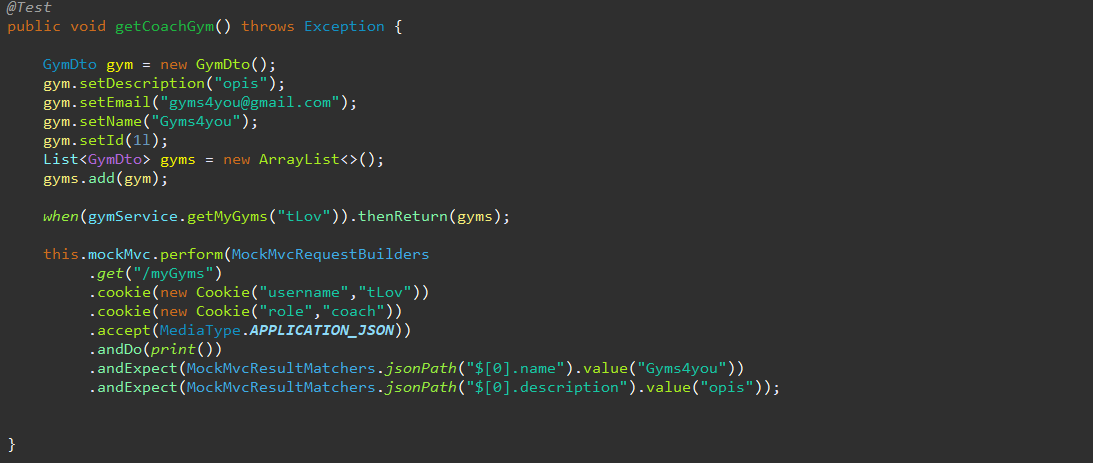
\includegraphics[scale=0.5]{slike/getCoachGym.PNG} %veličina slike u odnosu na originalnu datoteku i pozicija slike
    			\centering
    			\label{fig:promjene}
    	    \end{figure}
	
				
			\noindent \underbar{\textbf{4. Dohvati informacije o teretani}}
			
			Ovdje smo testirali pokušaj dohvaćanja informacija o određeneoj teretani odlaskom na /gymInfo sa pripadnim parametrom id koji se šalje preko URL-a.
             
			\begin{figure}[H]
    			\hspace*{-1.5cm}
    			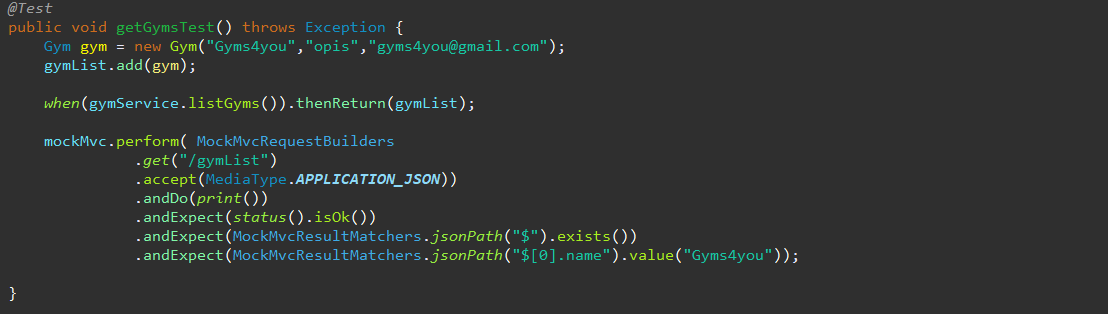
\includegraphics[scale=0.5]{slike/getGyms.PNG} %veličina slike u odnosu na originalnu datoteku i pozicija slike
    			\centering
    			\label{fig:promjene}
    	    \end{figure}
	

			\noindent \underbar{\textbf{5. Pronađi trenera}}
			
			Ovdje smo testirali pokušaj dohvaćanja trenera odlaskom na /coach sa pripadnim parametrom username koji se šalje preko URL-a.

			\begin{figure}[H]
    			\hspace*{-1.5cm}
    			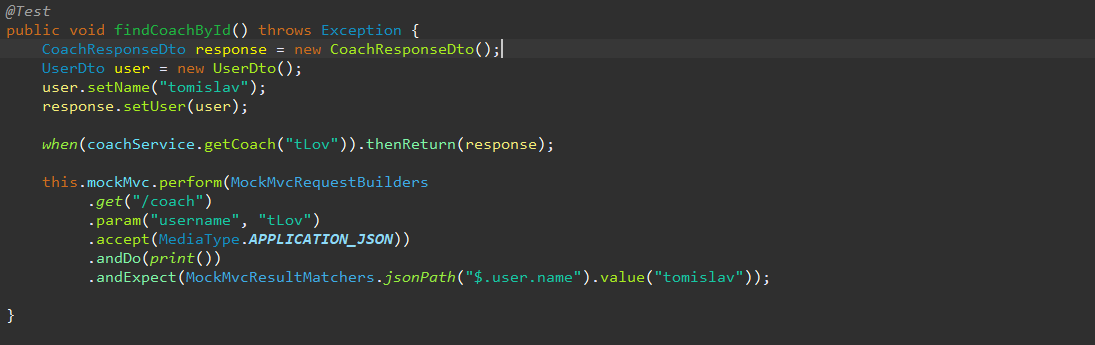
\includegraphics[scale=0.5]{slike/findCoachBy.PNG} %veličina slike u odnosu na originalnu datoteku i pozicija slike
    			\centering
    			\label{fig:promjene}
    	    \end{figure}
	

				
			\noindent \underbar{\textbf{6. Pronađi trenera (error) }}
			
			 Ovdje smo testirali pokušaj dohvaćanja trenera odlaskom na /coach bez parametra username kako bi dobili response 4xx koji javlja da je došlo do pogreške.
			\begin{figure}[H]
    			\hspace*{-1.5cm}
    			
\includegraphics[scale=0.5]{slike/findCoachByError.PNG} %veličina slike u odnosu na originalnu datoteku i pozicija slike
    			\centering
    			\label{fig:promjene}
    	    \end{figure}
	

				
			\noindent \underbar{\textbf{Prikaz prolaza svih ispita}}

			\begin{figure}[H]
    			\hspace*{-1.5cm}
    			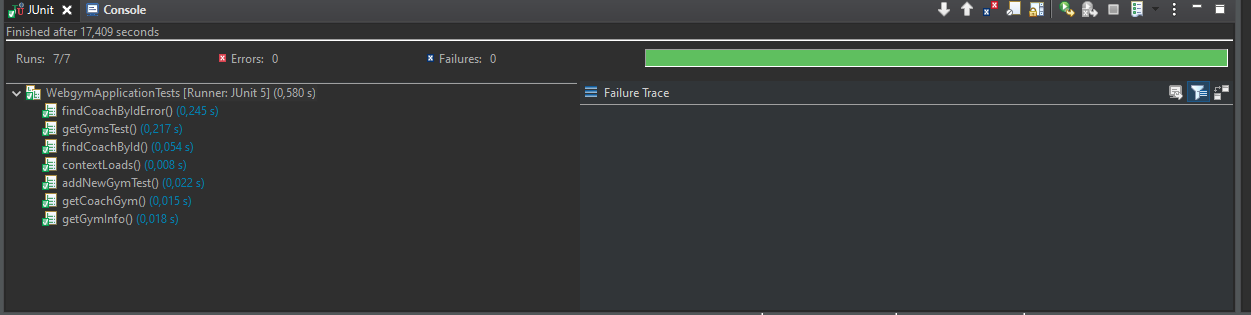
\includegraphics[scale=0.5]{slike/rezultati.PNG} %veličina slike u odnosu na originalnu datoteku i pozicija slike
    			\centering
    			\label{fig:promjene}
    	    \end{figure}
	

			\subsection{Ispitivanje sustava}
			
			 \textit{Potrebno je provesti i opisati ispitivanje sustava koristeći radni okvir . Razraditi \textbf{minimalno 4 ispitna slučaja} u kojima će se ispitati redovni slučajevi, rubni uvjeti te poziv funkcionalnosti koja nije implementirana/izaziva pogrešku kako bi se vidjelo na koji način sustav reagira kada nešto nije u potpunosti ostvareno. Ispitni slučaj se treba sastojati od ulaza (npr. korisničko ime i lozinka), očekivanog izlaza ili rezultata, koraka ispitivanja i dobivenog izlaza ili rezultata.\\ }
			 
		
		 	 Za ispitivanje funkcionalnosti sustava koristili smo Selenium IDE. Testirali smo
		 	 sve obrazce uporabe te smo prolazili kroz aplikaciju i gledali općenito ponašanje
		 	 u nadi da pronađemo neko neočekivano hazardno ponašanje u svrhu otklonuća problema.
		 	 Neke od testiranih obrazaca uporabe smo prikazali u nastavku. ( UC1, UC2, UC3, UC7).
		 	 
		 	 
	
	            \noindent \underbar{\textbf{1. Ispitni slučaj (UC1 : Pregled teretana)}}
                \begin{packed_item}
						\item  \textbf{Ulaz : } 
						\item[] \begin{packed_enum}
	
							\item korisnik je pritisnuo na "popis teretana"

						\end{packed_enum}
						\item  \textbf{Očekivani rezultat: } 
						\item[] \begin{packed_enum}
	
							\item korisnik je dobio prikaz svih teretana

						\end{packed_enum}
						
						\item  \textbf{rezultat : }
						\item[] \begin{packed_enum}
	
							\item rezultat je jednak očekivanom rezultatu.

						\end{packed_enum}

				\end{packed_item}
				
				\begin{figure}[H]
        			\hspace*{-1.5cm}
        			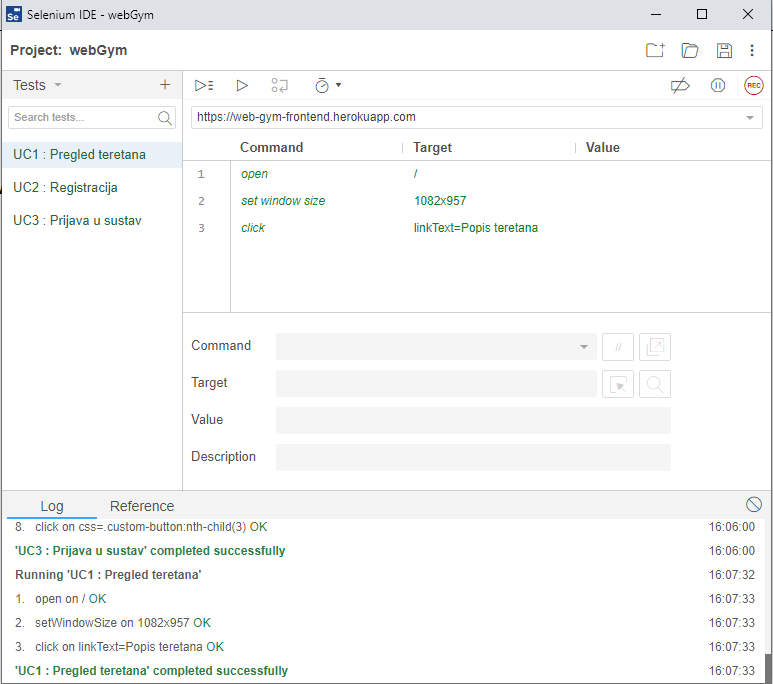
\includegraphics[scale=0.5]{dijagrami/UC1.PNG} %veličina slike u odnosu na originalnu datoteku i pozicija slike
        			\centering
        			\label{fig:promjene}
	        	\end{figure}
				
				\noindent \underbar{\textbf{2. Ispitni slučaj (UC2 : Registracija korisnika)}}
                \begin{packed_item}
						\item  \textbf{Ulaz : } 
						\item[] \begin{packed_enum}
	
							\item korisnik je pritisnuo na "prijava"
							\item korisnik je ispunio obrazac "registracija"
							\item korisnik je pritisnuo "registriraj"

						\end{packed_enum}
						\item  \textbf{Očekivani rezultat: } 
						\item[] \begin{packed_enum}
	
							\item korisnik se uspješno registrirao i spremio u bazu podataka

						\end{packed_enum}
						
						\item  \textbf{rezultat : }
						\item[] \begin{packed_enum}
	
							\item rezultat je jednak očekivanom rezultatu.

						\end{packed_enum}

				\end{packed_item}
				
				\begin{figure}[H]
        			\hspace*{-1.5cm}
        			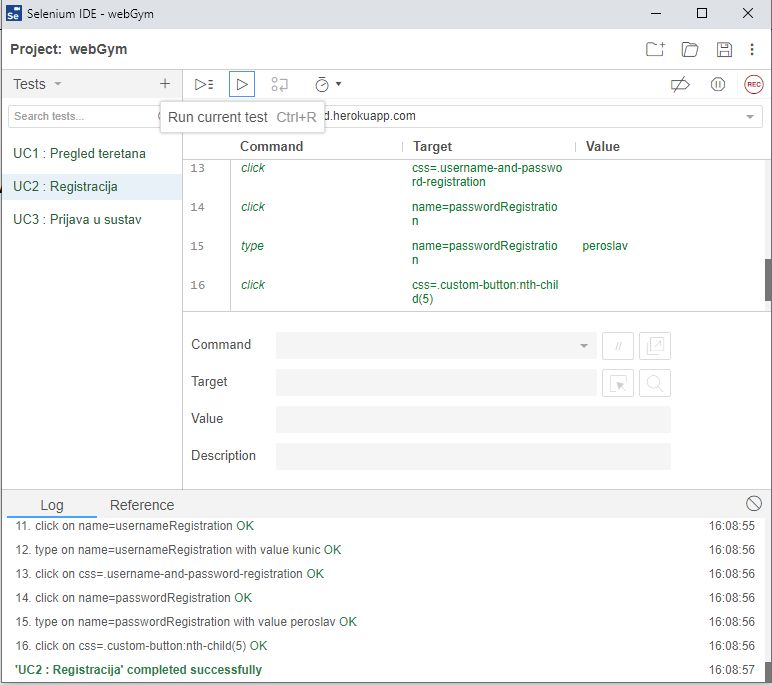
\includegraphics[scale=0.5]{dijagrami/UC2.PNG} %veličina slike u odnosu na originalnu datoteku i pozicija slike
        			\centering
        			\label{fig:promjene}
	        	\end{figure}
				
				\noindent \underbar{\textbf{3. Ispitni slučaj (UC3 : Prijava u sustav)}}
                \begin{packed_item}
						\item  \textbf{Ulaz : } 
						\item[] \begin{packed_enum}
	
							\item korisnik je pritisnuo na "prijava"
							\item korisnik je ispunio obrazac "prijava"
							\item korisnik je pritisnuo "prijava"

						\end{packed_enum}
						\item  \textbf{Očekivani rezultat: } 
						\item[] \begin{packed_enum}
	
							\item korisnik se uspješno prijavio u sustav

						\end{packed_enum}
						
						\item  \textbf{rezultat : }
						\item[] \begin{packed_enum}
	
							\item rezultat je jednak očekivanom rezultatu.

						\end{packed_enum}

				\end{packed_item}
				
				\begin{figure}[H]
        			\hspace*{-1.5cm}
        			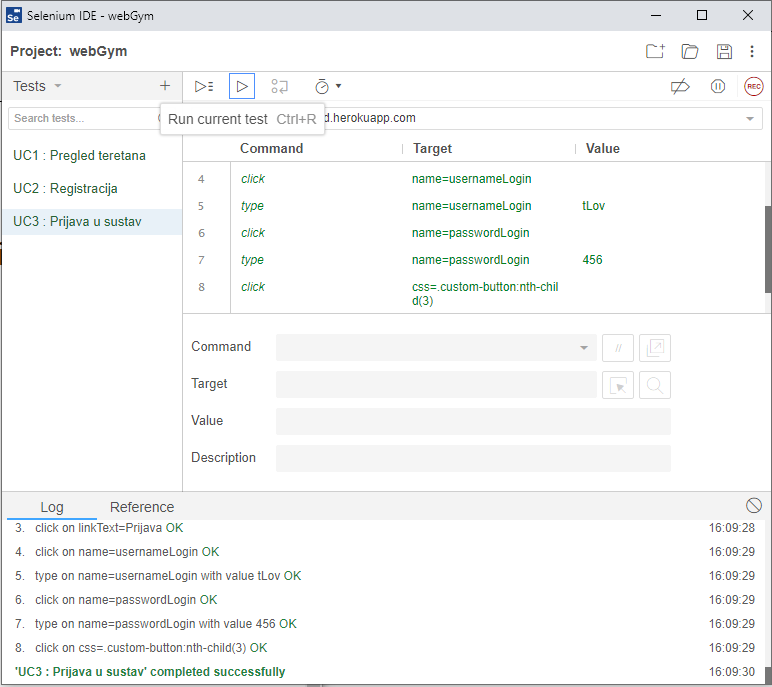
\includegraphics[scale=0.5]{dijagrami/UC3.PNG} %veličina slike u odnosu na originalnu datoteku i pozicija slike
        			\centering
        			\label{fig:promjene}
	        	\end{figure}
				
				\noindent \underbar{\textbf{4. Ispitni slučaj (UC7 : Pregled specifične teretane)}}
                \begin{packed_item}
						\item  \textbf{Ulaz : } 
						\item[] \begin{packed_enum}
	
							\item korisnik je pritisnuo na "Popis teretana"
							
							\item korisnik je pritisnuo na gumb informacije

						\end{packed_enum}
						\item  \textbf{Očekivani rezultat: } 
						\item[] \begin{packed_enum}
	
							\item korisnik je dobio informacije o odabranoj teretani

						\end{packed_enum}
						
						\item  \textbf{rezultat : }
						\item[] \begin{packed_enum}
	
							\item rezultat je jednak očekivanom rezultatu.

						\end{packed_enum}

				\end{packed_item}
					\begin{figure}[H]
        			\hspace*{-1.5cm}
        			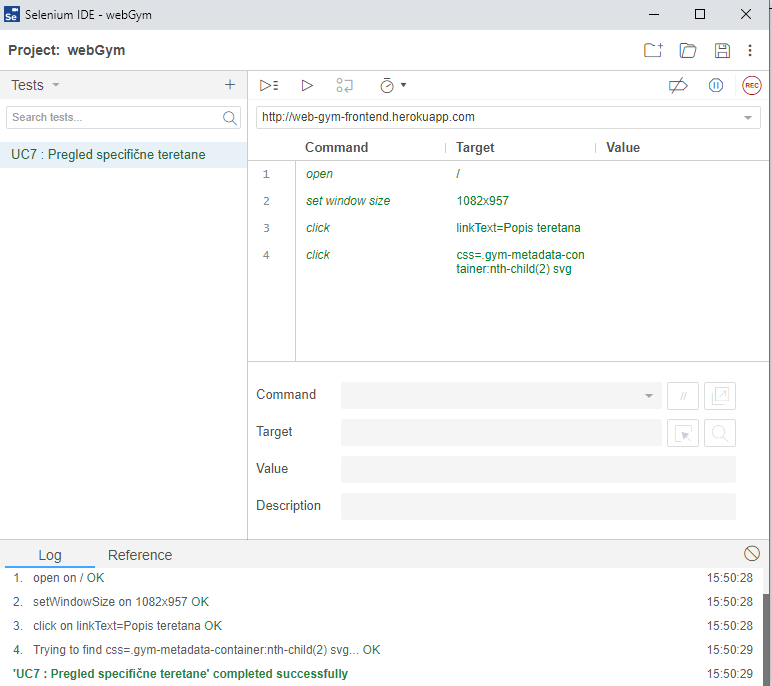
\includegraphics[scale=0.5]{slike/teretana.PNG} %veličina slike u odnosu na originalnu datoteku i pozicija slike
        			\centering
        			\label{fig:promjene}
	        	\end{figure}
	        	
	        \noindent \underbar{\textbf{5. Ispitni slučaj (UC20 : Pregled trenereove ponude)}}
                \begin{packed_item}
						\item  \textbf{Ulaz : } 
						\item[] \begin{packed_enum}
	
							\item trener je pritisnuo na "Moji planovi"

						\end{packed_enum}
						\item  \textbf{Očekivani rezultat: } 
						\item[] \begin{packed_enum}
	
							\item trener je dobio prikaz svih svojih planova treninga

						\end{packed_enum}
						
						\item  \textbf{rezultat : }
						\item[] \begin{packed_enum}
	
							\item došlo je do pogreške te se nisu učitali trenerovi planovi.
                                                
                            - Test je napravljen prije implementiranja mogućnosti trenera da pregleda svoje planove treninga i prehrane , do greške je došlo zbog problema u pamćenju cookie-a koje smo naknadno riješili.
                        
						\end{packed_enum}

				\end{packed_item}
					\begin{figure}[H]
        			\hspace*{-1.5cm}
        			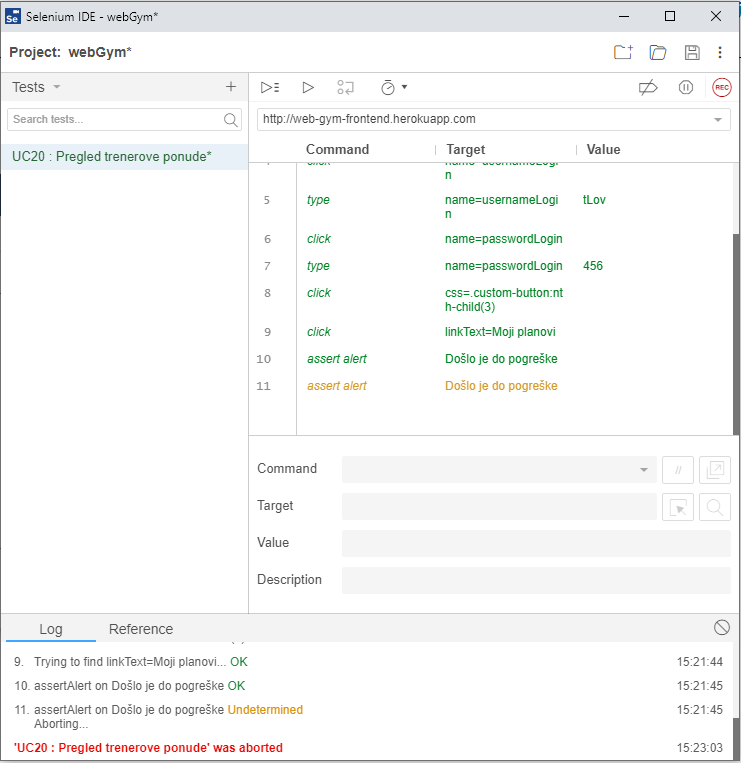
\includegraphics[scale=0.5]{slike/error.PNG} %veličina slike u odnosu na originalnu datoteku i pozicija slike
        			\centering
        			\label{fig:promjene}
	        	\end{figure}
		 
			\eject 
			
			
		\section{Dijagram razmještaja}
		
		 \textit{Potrebno je umetnuti \textbf{specifikacijski} dijagram razmještaja i opisati ga. Moguće je umjesto specifikacijskog dijagrama razmještaja umetnuti dijagram razmještaja instanci, pod uvjetom da taj dijagram bolje opisuje neki važniji dio sustava.}
		
		Dijagram razmještaja prikazuje generalnu topologiju sustava koji se koristi kako bi resursi bili optimalno raspoređeni. Predstavlja statički pogled na razmještaj sklopovskih i programskih komponenata. Na poslužiteljskom računalu se nalaze web poslužitelj, poslužitelj baze podataka i poslužitelj za frontend. Klijenti koriste web preglednik kako bi pristupili web aplikaciji. U bazi podataka sadržane su sve potrebne informacije i datoteke koje korisnik može zahtijevati. Sustav je baziran na arhitekturi ”klijent – poslužitelj”. Komunikacija između poslužiteljskog računala i klijentskog računala se omogućuje HTTP protokolom. 
		
		
		
		\begin{figure}[h]
			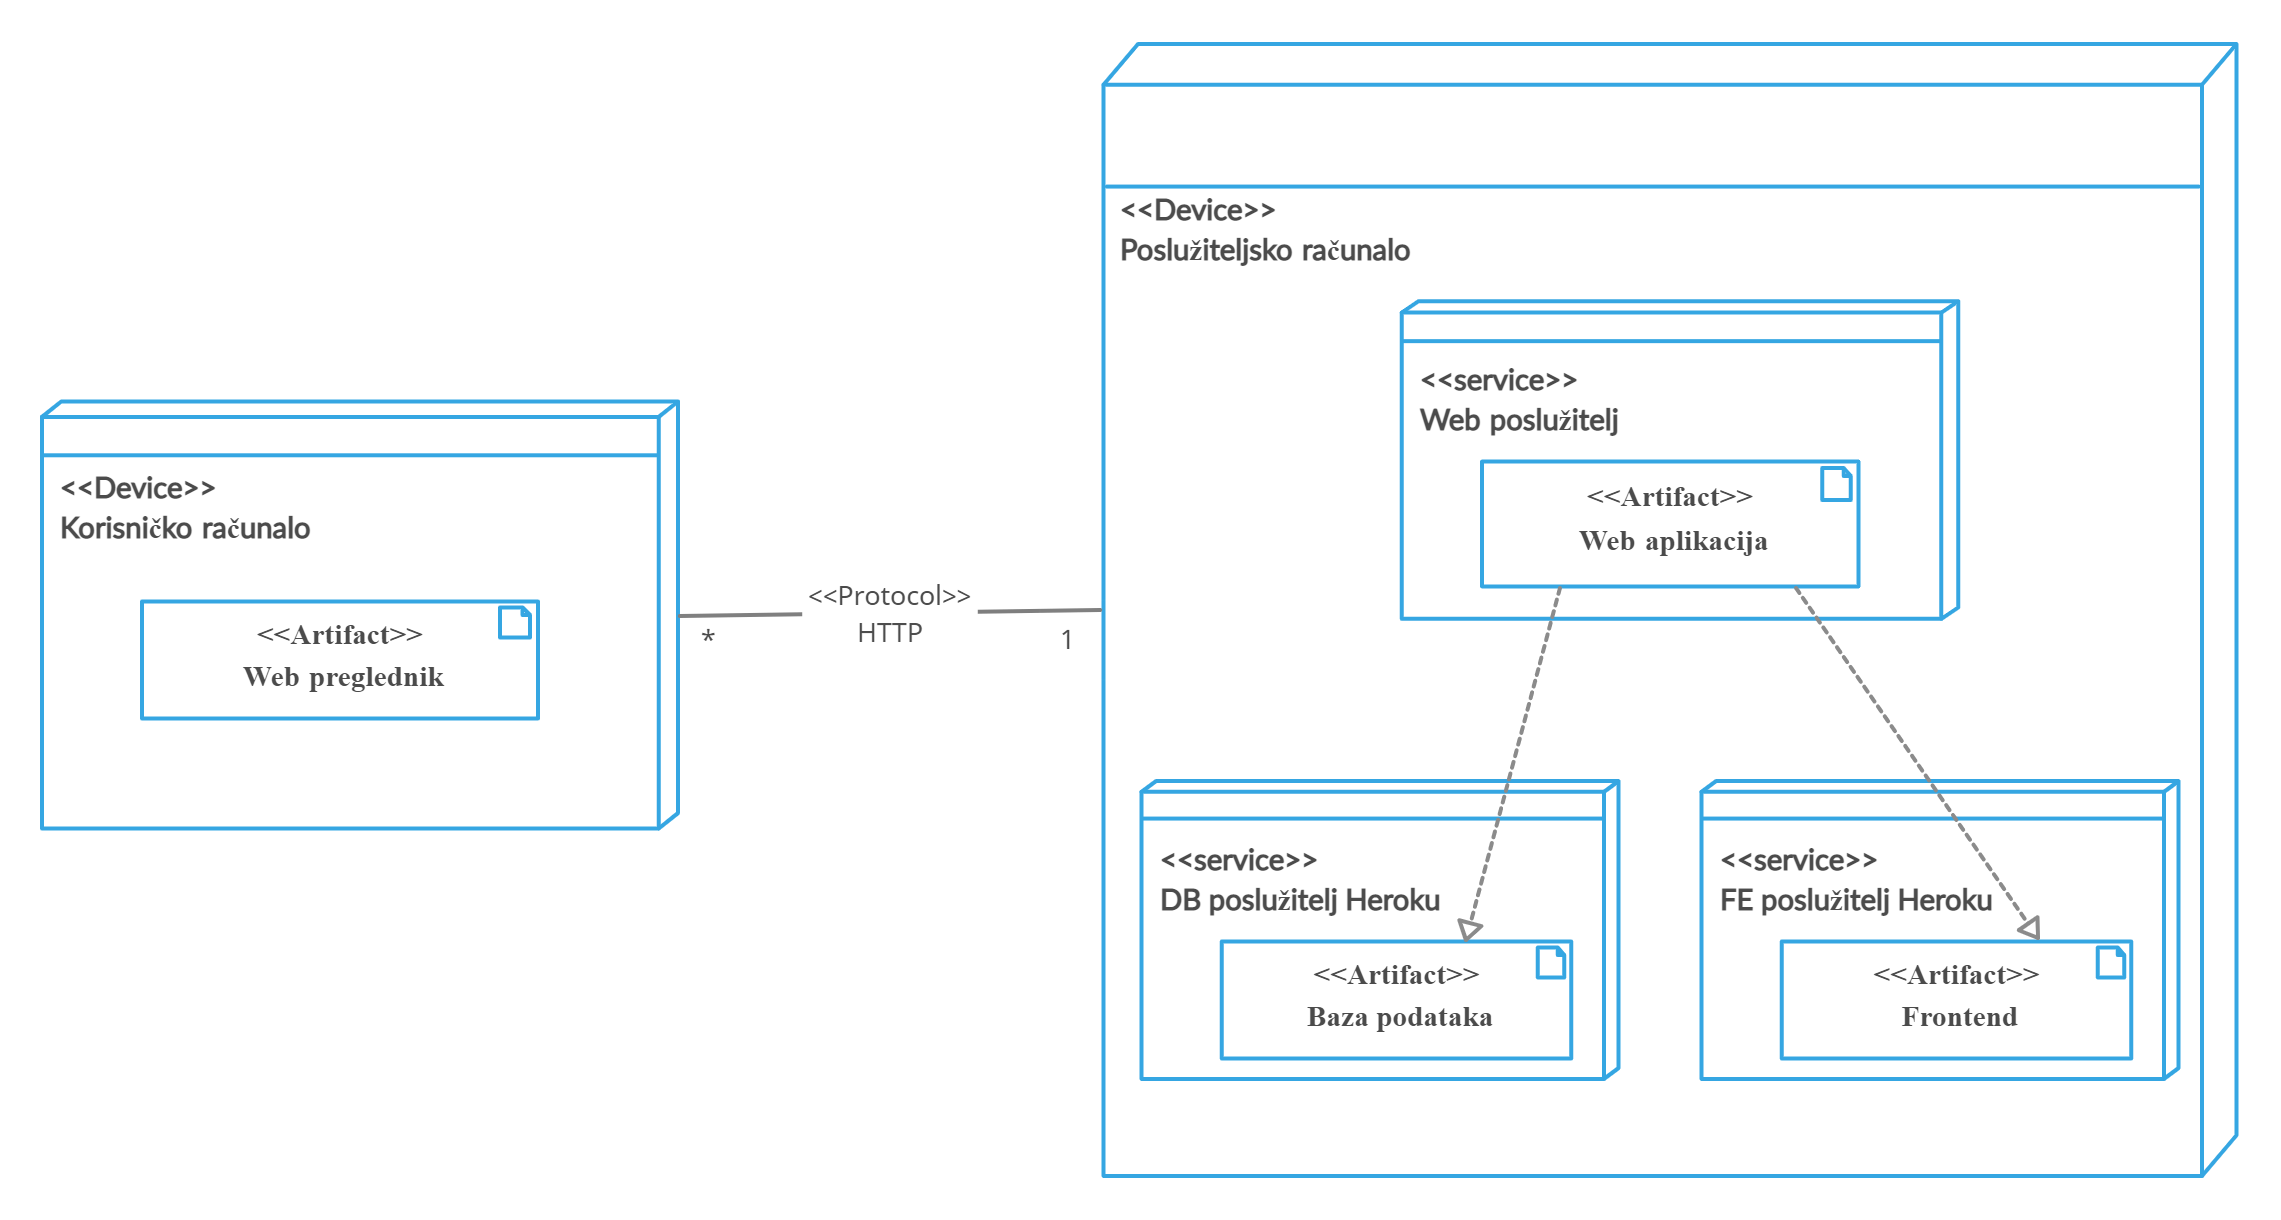
\includegraphics[height=                       9cm,width=1\textwidth]{dijagrami/Dijagram_razmjestaja.png}
			\begin{center}
				Slika 5.1: Dijagram razmještaja
			\end{center}
		\end{figure}
		
		\eject	
		
		
		\section{Upute za puštanje u pogon}

		    \begin{packed_item}
						\item  \textbf{1. Stvaranje backend heroku servera} 
						\item[] \begin{packed_enum}
	
							\item Stvaranje account-a na https://dashboard.heroku.com/
							
							\item Instalacija Heroku CLI : https://devcenter.heroku.com/articles/heroku-cli
							
							\item Otvaranje command prompt-a
							
							\item Upiši "heroku create "NAME-OF-APP" (webGym) ili samo "heroku create"
							
							    - U slučaju da se ne navede ime aplikacije , i dalje će se stvoriti server ali s random imenom koji je kasnije moguće preimenovati u željeno ime.
							
							\item Stvoren je server.
							    
							    \begin{figure}[H]
                        			\hspace*{-1.5cm}
                        			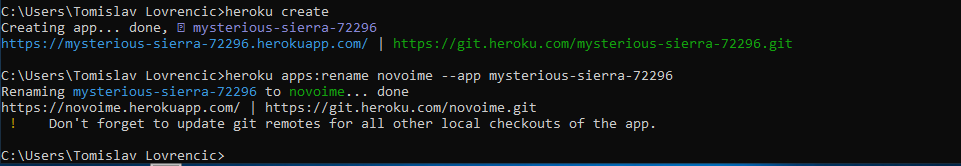
\includegraphics[scale=0.5]{dijagrami/cmd.PNG} %veličina slike u odnosu na originalnu datoteku i pozicija slike
                        			\centering
                        			\label{fig:promjene}
                        		\end{figure}

						\end{packed_enum}
						\item  \textbf{2. Konfiguracija baze podataka} 
						\item[] \begin{packed_enum}
	
							\item Odlazak na stranicu  https://dashboard.heroku.com/
							
							\item Klik na stvoreni server. (novoime)
							
							\item Klik na resources
							
							\item Pronaći pod add-ons  Heroku POSTGRES
							
							    - Odabrati Hobby dev - FREE
							  
							
							\item Stisnuti na SUBMIT FORM.
							
							\item Stvorena je baza podataka
							    
							    \begin{figure}[H]
                        			\hspace*{-1.5cm}
                        			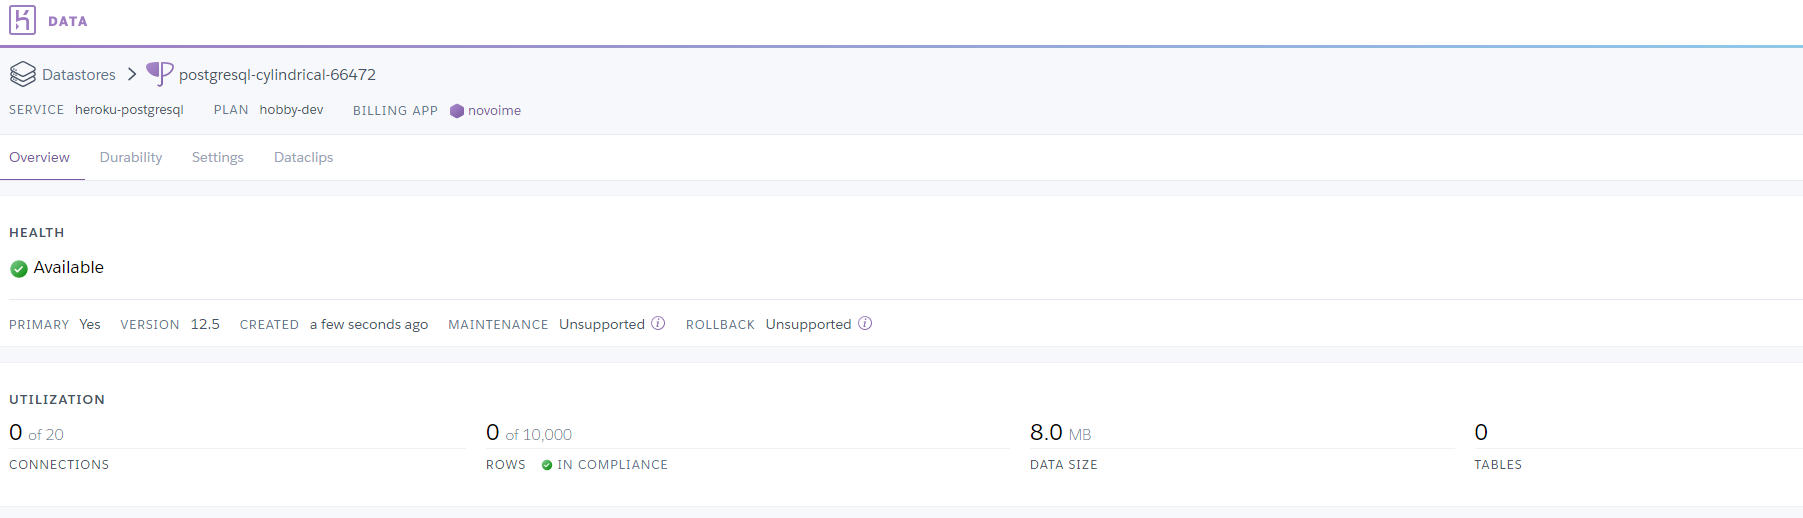
\includegraphics[scale=0.3]{dijagrami/baza.PNG} %veličina slike u odnosu na originalnu datoteku i pozicija slike
                        			\centering
                        			\label{fig:promjene}
                        		\end{figure}

						\end{packed_enum}
						
						
						\item  \textbf{3. Spajanje backend server na stvorenu bazu u heroku}
						\item[] \begin{packed_enum}
	
							\item Odlazak na stranicu  https://dashboard.heroku.com/
							
							\item Klik na stvoreni server. (novoime)
							
							\item Klik na resources
							
							\item Klik na Heroku POSTGRES
							
							\item Klik na settings
							
							\item Klik na view credentials
							
							\item Otvori backend kod (java)
							
							\item Odi u src/main/resources/application.properties
							
							\item Podesi :
							    
							       - Potrebno je podesiti backend tako da se povezuje sa bazom koju smo u prethodnom koraku stvorili na heroku.
							       
							       - U tom naumu ćemo morati podesiti spring.datasource.url , spring.datasource.username te spring.datasource.password na način da ćemo pročitati vrijednosti koje nam je dao heroku credentials i nadodati ih na spomenute vrijednosti.
							       
							       - Zadnja napomena je dodavanje "jdbc:" na početak URI-a koje nam je generirao heroku.
						
							    \begin{figure}[H]
                        			\hspace*{-1.5cm}
                        			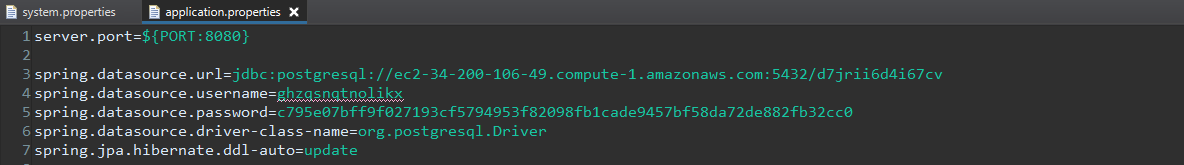
\includegraphics[scale=0.5]{slike/java.PNG} %veličina slike u odnosu na originalnu datoteku i pozicija slike
                        			\centering
                        			\label{fig:promjene}
                        		\end{figure}

						\end{packed_enum}
						
						\item  \textbf{4. deploy backend-a}
						\item[] \begin{packed_enum}
	
							\item Otvoriti backend project.
							
							\item Otvoriti pom.xml te dodati ovaj plugin.
			
							    \begin{figure}[H]
                        			\hspace*{-1.5cm}
                        			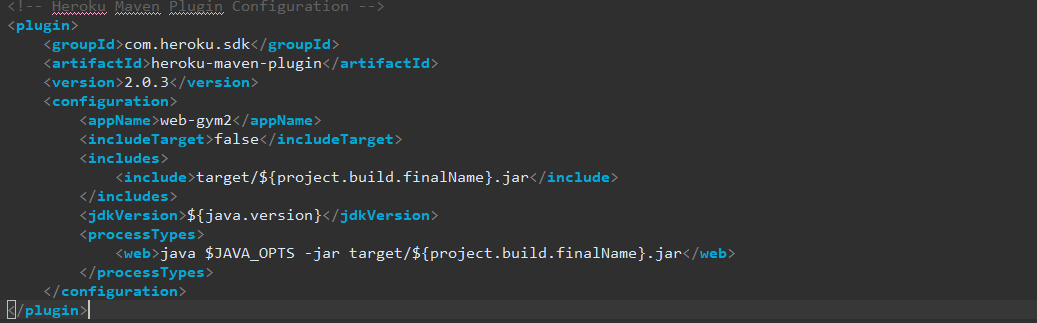
\includegraphics[scale=0.5]{slike/plugin.PNG} %veličina slike u odnosu na originalnu datoteku i pozicija slike
                        			\centering
                        			\label{fig:promjene}
                        		\end{figure}
                        		
                        		- Napomena : u našem slučaju prateći sve ove korake bi treabli napisati
                        		pod appName "novoime", dok nam je za projekt ime aplikacije ,kao što možemo vidjeti na slici "web-gym2".
							
							\item Otvoriti cmd te se pozicionirati u root backend projekta
							
							\item Napisati "mvn clean heroku:deploy"
						

						\end{packed_enum}
						
				\item  \textbf{5. Stvaranje frontend servera te deploy frontend-a}
				\item[] \begin{packed_enum}
	
							\item Odlazak na stranicu  https://dashboard.heroku.com/
							
							\item Otvoriti cmd te upisati "heroku create NAME-OF-FRONTEND-APP --buildpack https://github.com/mars/create-react-app-buildpack.git"

							\item Napraviti prazan folder , unutar foldera u cmd-u napisati "git init"
							
							\item U cmd-u napisati "heroku git:remote -a NAME-OF-FRONTEND-APP"
							
							\item Prekopirati root frontend projekta u stvoreni folder
							
							\item Dodati static.json datoteku u root frontend projekta
							    
							    \begin{figure}[H]
                        			\hspace*{-1.5cm}
                        			
\includegraphics[scale=0.5]{slike/json.PNG} %veličina slike u odnosu na originalnu datoteku i pozicija slike
                        			\centering
                        			\label{fig:promjene}
                        		\end{figure}
							
							\item prije deploya frontenda , ući u src/App.js te promjeniti backendURL i 
							postaviti ga na server backenda.
							
							    \begin{figure}[H]
                        			\hspace*{-1.5cm}
                        			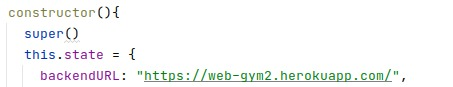
\includegraphics[scale=0.7]{slike/front.png} %veličina slike u odnosu na originalnu datoteku i pozicija slike
                        			\centering
                        			\label{fig:promjene}
                        		\end{figure}
							
							\item U cmd- napisati "git add ."
							
							\item U cmd- napisati "git add -m "initial commit""
							
							\item U cmd- napisati "git push heroku master"
	

						\end{packed_enum}

				\end{packed_item}
				
			\eject 
	\chapter{Zaključak i budući rad}
		
		\textbf{\textit{dio 2. revizije}}\\
		
		 \textit{U ovom poglavlju potrebno je napisati osvrt na vrijeme izrade projektnog zadatka, koji su tehnički izazovi prepoznati, jesu li riješeni ili kako bi mogli biti riješeni, koja su znanja stečena pri izradi projekta, koja bi znanja bila posebno potrebna za brže i kvalitetnije ostvarenje projekta i koje bi bile perspektive za nastavak rada u projektnoj grupi.}
		
		 \textit{Potrebno je točno popisati funkcionalnosti koje nisu implementirane u ostvarenoj aplikaciji.}
		
		\eject 
	\chapter*{Popis literature}
		\addcontentsline{toc}{chapter}{Popis literature}
	 	
 		\textbf{\textit{Kontinuirano osvježavanje}}
	
		\textit{Popisati sve reference i literaturu koja je pomogla pri ostvarivanju projekta.}
		
		
		\begin{enumerate}
			
			
			\item  Programsko inženjerstvo, FER ZEMRIS, \url{http://www.fer.hr/predmet/proinz}
			
			\item  I. Sommerville, "Software engineering", 8th ed, Addison Wesley, 2007.
			
			\item  T.C.Lethbridge, R.Langaniere, "Object-Oriented Software Engineering", 2nd ed. McGraw-Hill, 2005.
			
			\item  I. Marsic, Software engineering book``, Department of Electrical and Computer Engineering, Rutgers University, \url{http://www.ece.rutgers.edu/~marsic/books/SE}
			
			\item  The Unified Modeling Language, \url{https://www.uml-diagrams.org/}
			
			\item  Astah Community, \url{http://astah.net/editions/uml-new}
		\end{enumerate}
		
		 
	
	
	\begingroup
	\renewcommand*\listfigurename{Indeks slika i dijagrama}
	%\renewcommand*\listtablename{Indeks tablica}
	%\let\clearpage\relax
	\listoffigures
	%\vspace{10mm}
	%\listoftables
	\endgroup
	\addcontentsline{toc}{chapter}{Indeks slika i dijagrama}


	
	\eject 
		
	\chapter*{Dodatak: Prikaz aktivnosti grupe}
		\addcontentsline{toc}{chapter}{Dodatak: Prikaz aktivnosti grupe}
		
		\section*{Dnevnik sastajanja}
		
		\textbf{\textit{Kontinuirano osvježavanje}}\\
		
		 \textit{U ovom dijelu potrebno je redovito osvježavati dnevnik sastajanja prema predlošku.}
		
		\begin{packed_enum}
			\item  sastanak
			
			\item[] \begin{packed_item}
				\item 7.listopada 2020.
				\item Prisustvovali: L.Merćep, J.Milić, E.Đuras, F.Sodić, D.Kniewald, T.Lovrenčić, B.Dević
				\item Teme sastanka:
				\begin{packed_item}
					\item  Inicijalna pitanja asistentu za projekt
				\end{packed_item}
			\end{packed_item}
			
			\item  sastanak
			\item[] \begin{packed_item}
				\item 14.listopada 2020.
				\item Prisustvovali: L.Merćep, J.Milić, E.Đuras, F.Sodić, D.Kniewald, T.Lovrenčić, B.Dević
				\item Teme sastanka:
				\begin{packed_item}
					\item  Podjela tima na backend i frontend
				\end{packed_item}
			\end{packed_item}
			
			\item  sastanak
			\item[] \begin{packed_item}
				\item 20.listopada 2020.
				\item Prisustvovali: E.Đuras, F.Sodić, D.Kniewald
				\item Teme sastanka:
				\begin{packed_item}
					\item  Frontend
					\item  Istraživanje react tehnologije
				\end{packed_item}
			\end{packed_item}
			
			\item  sastanak
			\item[] \begin{packed_item}
				\item 24.listopada 2020.
				\item Prisustvovali: L.Merćep, J.Milić, T.Lovrenčić, B.Dević
				\item Teme sastanka:
				\begin{packed_item}
					\item  Backend
					\item  Istraživanje Spring Boot i Heroku tehnologija
				\end{packed_item}
			\end{packed_item}
			
			\item  sastanak
			\item[] \begin{packed_item}
				\item 30.listopada 2020.
				\item Prisustvovali: L.Merćep, J.Milić, D.Kniewald, T.Lovrenčić
				\item Teme sastanka:
				\begin{packed_item}
					\item  Dokumentacija
					\item Revizija Funkcionalnih zahtjeva koje je F.Sodić napisao
					\item Obrasci uporabe
				\end{packed_item}
			\end{packed_item}
			
			%
			
		\end{packed_enum}
		
		\eject
		\section*{Tablica aktivnosti}
		
			\textbf{\textit{Kontinuirano osvježavanje}}\\
			
			 \textit{Napomena: Doprinose u aktivnostima treba navesti u satima po članovima grupe po aktivnosti.}
					
						
			
			\begin{longtabu} to \textwidth {|X[7, l]|X[1, c]|X[1, c]|X[1, c]|X[1, c]|X[1, c]|X[1, c]|X[1, c]|}
								
				\cline{2-8} \multicolumn{1}{c|}{\textbf{}} &     \multicolumn{1}{c|}{\rotatebox{90}{\textbf{Luka Merćep }}} & \multicolumn{1}{c|}{\rotatebox{90}{\textbf{Jura Milić }}} &	\multicolumn{1}{c|}{\rotatebox{90}{\textbf{Eduard Đuras }}} &	\multicolumn{1}{c|}{\rotatebox{90}{\textbf{Fran Sodić }}} &
				\multicolumn{1}{c|}{\rotatebox{90}{\textbf{Dominik Kniewald }}} &
				\multicolumn{1}{c|}{\rotatebox{90}{\textbf{Tomislav Lovrenčić }}} &	\multicolumn{1}{c|}{\rotatebox{90}{\textbf{Bruno Dević }}} \\ \hline 
				\endfirsthead
				
			
				\cline{2-8} \multicolumn{1}{c|}{\textbf{}} &     \multicolumn{1}{c|}{\rotatebox{90}{\textbf{Luka Merćep}}} & \multicolumn{1}{c|}{\rotatebox{90}{\textbf{Jura Milić }}} &	\multicolumn{1}{c|}{\rotatebox{90}{\textbf{Eduard Đuras }}} &
				\multicolumn{1}{c|}{\rotatebox{90}{\textbf{Fran Sodić }}} &	\multicolumn{1}{c|}{\rotatebox{90}{\textbf{Dominik Kniewald }}} &
				\multicolumn{1}{c|}{\rotatebox{90}{\textbf{Tomislav Lovrenčić }}} &	\multicolumn{1}{c|}{\rotatebox{90}{\textbf{Bruno Dević }}} \\ \hline 
				\endhead
				
				
				\endfoot
							
				 
				\endlastfoot
				
				Upravljanje projektom 	     & 7 &  & 3 &  &  &  & \\ \hline
				Opis projektnog zadatka 	 & 5 &  &  &  &  &  & \\ \hline
				
				Funkcionalni zahtjevi       &  &  &  & 5 &  &  &  \\ \hline
				Opis pojedinih obrazaca 	& 3 & 3 &  &  & 5 & 5 &  \\ \hline
				Dijagram obrazaca 			&  &  &  &  &  & 4 &  \\ \hline
				Sekvencijski dijagrami 		&  &  &  &  &  &  & 4  \\ \hline
				Opis ostalih zahtjeva 		&  &  &  &  & 2 &  &  \\ \hline

				Arhitektura i dizajn sustava	 &  &  & 2 &  &  &  & 3 \\ \hline
				Baza podataka				 & 3 &  &  & 2 & 2 & 4 & 4  \\ \hline
				Dijagram razreda 			& 2 &  &  &  &  & 5 &   \\ \hline
				Dijagram stanja				&  &  &  &  &  &  &  \\ \hline
				Dijagram aktivnosti 		&  &  &  &  &  &  &  \\ \hline
				Dijagram komponenti			&  &  &  &  &  &  &  \\ \hline
				Korištene tehnologije i alati 		&  &  &  &  &  &  &  \\ \hline
				Ispitivanje programskog rješenja 	&  &  &  &  &  &  &  \\ \hline
				Dijagram razmještaja			&  &  &  &  &  &  &  \\ \hline
				Upute za puštanje u pogon 		&  &  &  &  &  &  &  \\ \hline 
				Dnevnik sastajanja 			&  &  &  &  &  &  &  \\ \hline
				Zaključak i budući rad 		&  &  &  &  &  &  &  \\  \hline
				Popis literature 			&  &  &  &  &  &  &  \\  \hline
				&  &  &  &  &  &  &  \\ \hline \hline
				{Dodatne stavke kako ste podijelili izradu aplikacije} 			&  &  &  &  &  &  &  \\ \hline
				{Izrada početne stranice} 				&  &  & 15 & 7 &  &  &  \\ \hline 
				{Izrada baze podataka} 		 			&  & 5 &  &  &  &  & \\ \hline 
				{Spajanje s bazom podataka} 							&  & 4 &  &  &  & 2 &  \\ \hline
				{Back end} 							&  & 5 &  &  &  &  &  \\  \hline
				{Čitanje i provjera dokumentacije} 							&  &  &  & 5 & 2 &  &  \\  \hline
				 							&  &  &  &  &  &  &\\  \hline
				
				
			\end{longtabu}
					
					
		\eject
		\section*{Dijagrami pregleda promjena}
		
		\textbf{\textit{dio 2. revizije}}\\
		
		\textit{Prenijeti dijagram pregleda promjena nad datotekama projekta. Potrebno je na kraju projekta generirane grafove s gitlaba prenijeti u ovo poglavlje dokumentacije. Dijagrami za vlastiti projekt se mogu preuzeti s gitlab.com stranice, u izborniku Repository, pritiskom na stavku Contributors.}
		
	


\end{document} %naredbe i tekst nakon ove naredbe ne ulaze u izgrađen dokument 


